%%%%%%%%%%%
% Todo: cluster locations using decision trees for actions and/or transitions? Gives a grid!
%- use decision tree for personalizing?
%- redo value iteration?
%

%%%%%%%%%%%%%%%%%%%%%%% file template.tex %%%%%%%%%%%%%%%%%%%%%%%%%
%
% This is a general template file for the LaTeX package SVJour3
% for Springer journals.          Springer Heidelberg 2010/09/16
%
% Copy it to a new file with a new name and use it as the basis
% for your article. Delete % signs as needed.
%
% This template includes a few options for different layouts and
% content for various journals. Please consult a previous issue of
% your journal as needed.
%
%%%%%%%%%%%%%%%%%%%%%%%%%%%%%%%%%%%%%%%%%%%%%%%%%%%%%%%%%%%%%%%%%%%
%
% First comes an example EPS file -- just ignore it and
% proceed on the \documentclass line
% your LaTeX will extract the file if required
\begin{filecontents*}{example.eps}
%!PS-Adobe-3.0 EPSF-3.0
%%BoundingBox: 19 19 221 221
%%CreationDate: Mon Sep 29 1997
%%Creator: programmed by hand (JK)
%%EndComments
gsave
newpath
  20 20 moveto
  20 220 lineto
  220 220 lineto
  220 20 lineto
closepath
2 setlinewidth
gsave
  .4 setgray fill
grestore
stroke
grestore
\end{filecontents*}
%
\RequirePackage{fix-cm}
%
%\documentclass{svjour3}                     % onecolumn (standard format)
%\documentclass[smallcondensed]{svjour3}     % onecolumn (ditto)
\documentclass[smallextended]{svjour3}       % onecolumn (second format)
%\documentclass[twocolumn]{svjour3}          % twocolumn
%
\smartqed  % flush right qed marks, e.g. at end of proof
%
\usepackage{graphicx}
\usepackage{multirow}
%\usepackage{subcaption}

%\usepackage{cleveref}
%
% \usepackage{mathptmx}      % use Times fonts if available on your TeX system
%
% insert here the call for the packages your document requires
%\usepackage{latexsym}
% etc.
%
% please place your own definitions here and don't use \def but
% \newcommand{}{}
%
% Insert the name of "your journal" with
\journalname{Data Mining and Knowledge Discovery}
%
%\usepackage{subfigure}

%\usepackage{proceed2e}
\usepackage{booktabs} 
% Set the typeface to Times Roman
\usepackage{times}
\usepackage{url}
\usepackage[square]{natbib}
\usepackage{varwidth}
%Example for automatically rescaling equations. 
% This is very tricky.
%\begin{equation}
%\label{eq:pimax}
%\resizebox{.55\textwidth}{!}{$
%\begin{split}
%P(\jtable_{2}|\set{E},\ttable) \propto &
%P(\keys = [jack,101],\it{Gr} = A, \it{Sat} = 1|\it{Int} = \class, \it{Rank} = 1, \it{Rat} = 3, \it{Diff}=1)\\
%\times & P(\keys = [jack,102],\it{Gr} = B, \it{Sat} = 2|\it{Int} = \class, \it{Rank} = 1, \it{Rat} = 2, \it{Diff}=2).
%\end{split}$
%}
%\end{equation}

%\usepackage{times}
%\usepackage[normaltitle,normalbib,normalmargins,normalindent]{savetrees}
\usepackage{amsmath}
\usepackage{amsfonts}
\usepackage{amssymb}
\usepackage{graphicx}
\usepackage{url}
%\usepackage{subfigure}
\usepackage{epstopdf}
\setcounter{MaxMatrixCols}{30}
%\usepackage{algorithm}
%\usepackage{algorithmic}
\usepackage{subfigure}
%\usepackage{subcaption}
\usepackage{fancyhdr}
\graphicspath{{../}{figures/}}
\usepackage{todonotes}

\DeclareMathOperator*{\argmax}{argmax}
\DeclareMathOperator*{\argmin}{argmin}
%\DeclareMathOperator{\pattern}{\pi}
\DeclareMathOperator{\Poly}{\mathbf{\mathrm{P}}}
\DeclareMathOperator{\RP}{\mathbf{\mathrm{RP}}}
%\DeclareMathOperator{\FP}{\mathbf{\mathrm{FP}}}
\DeclareMathOperator{\NP}{\mathbf{\mathrm{NP}}}
%\DeclareMathOperator{\E}{\mathbb{E}}
\renewcommand{\d}{\mathbf{d}}

\newcommand{\ZZ}{\mathbf{Z}}

\newcommand{\indep}{\ensuremath{\perp{}\!\!\!\!\!\!\!\perp{}}}
\newcommand{\dep}{\ensuremath{{\perp{}\!\!\!\!\!\!\!\not  \perp{}}}}
%\renewcommand{\L}{\mathcal{L}}
% variables denoting sets of nodes
\newcommand{\V}{V} 
\newcommand{\partC}{\mathcal{C}}
\newcommand{\pattern}{\pi}
% variables denoting nodes
\newcommand{\B}{B}
\renewcommand{\P}{P}
\newcommand{\R}{R}
\newcommand{\X}{X}
\newcommand{\Y}{Y}
\newcommand{\Z}{Z}
\newcommand{\F}{F}
\newcommand{\U}{U}
\newcommand{\W}{W}
\renewcommand{\S}{S}
\newcommand{\C}{C}
\newtheorem{mydef}{Proposition}
%variables for values
%\newcommand{\u}{u}
\renewcommand{\a}{a}
\renewcommand{\b}{b}
\newcommand{\z}{z}
\renewcommand{\v}{v}
\newcommand{\x}{x}
\newcommand{\y}{y}
\newcommand{\p}{p}
\newcommand{\s}{s}
\newcommand{\w}{w} % weights


%statistics
\newcommand{\divergence}{\it{D}}
\newcommand{\score}{\it{score}}
\newcommand{\confidence}{\it{conf}}
\newcommand{\support}{\it{support}}
\newcommand{\loglikelihood}{\it{LOG}}
\newcommand{\lof}{\it{LOF}}
\newcommand{\llmetric}{-L}
\newcommand{\lr}{\it{LR}}
\newcommand{\kl}{\it{KL}}
\newcommand{\el}{\it{EL}}
\newcommand{\mi}{\it{MI}}
\renewcommand{\mid}{\it{ELD}}
\newcommand{\jid}{\it{JID}}
\newcommand{\roc}{\it{ROC}}
\newcommand{\outrank}{\it{OutRank}}
\newcommand{\knn}{\it{KNNOutlier}}
\newcommand{\auc}{\it{AUC}}
\newcommand{\eld}{\it{ELD}}
\newcommand{\fd}{\it{FD}}
\newcommand{\parameter}{\theta}
\newcommand{\parameters}{\bs{\parameter}}
\newcommand{\bic}{\mathit{BIC}}
%random variables and graphical models
% number of values in the domain of a random variable
% variables for BNs
\newcommand{\domvals}{k}
\newcommand{\nodevalue}{\v}
\newcommand{\parvalue}{\mathbf{\pi}} % a single assignment of values to a set of 
%parents
\newcommand{\parvals}{l} % number of values of parent state.
\renewcommand{\r}{r} % CP-table row
\newcommand{\nbhd}{{\mathsf {nbdh}}}
\newcommand{\child}{\mathit{child}}
\newcommand{\parent}{\mathit{pa}}
\newcommand{\parents}{\mathbf{pa}}
\newcommand{\Parents}{\mathbf{PA}}
\newcommand{\family}{F} % families, family formulas
\newcommand{\vpi}{\mathbf{pa}} % for vectors of variable assignments
\renewcommand{\l}{\ell} % class label
\newcommand{\states}{r} % number of states of a variable
%\newcommand{\value}{value}
\newcommand{\mb}{\set{mb}} % markov blanket of a variable, vector-valued
\newcommand{\ssize}{N} % number of rows in join table; size of sample
\newcommand{\mbstates}{m} % number of states in Markov blanket
\newcommand{\frequency}{fr}
\newcommand{\pseudo}{\ast}
\newcommand{\counts}{+}
\newcommand{\weighted}{\ast}
\newcommand{\halpern}{H}
\newcommand{\Thetaa}{\theta}
\newcommand{\instance}{I}

%logic notation
%\newcommand{\predicate}{\phi}
\newcommand{\functor}{f}
\newcommand{\outdomain}{V}
\newcommand{\indomain}{\Omega}
\newcommand{\variable}{X} % first-order variable
\newcommand{\population}{\mathcal{P}}
\newcommand{\entity}{x}
\newcommand{\formula}{\phi}
\newcommand{\formulas}{\mathcal{\phi}}
\newcommand{\literal}{l}
\newcommand{\conjunction}{\set{C}} % conjunction of literals
\newcommand{\fterm}{\f} % open function term
\newcommand{\fterms}{F} % set of function terms, also nodes in JBN
\newcommand{\term}{\sigma}
\newcommand{\Terms}{\bs{\sigma}}
\newcommand{\constant}{a}
\newcommand{\constants}{\bs{\constant}}
\newcommand{\gterm}{g} % ground term
\newcommand{\gterms}{\bs{\gterm}} %list of ground terms
\newcommand{\vterm}{x} % variable term
\newcommand{\vterms}{\bs{\vterm}} % list of variable terms
\newcommand{\assign}{A} % assignment of values to Bayes net
\newcommand{\resultset}{\mathbb{R}}
\newcommand{\grounds}{\#}
\newcommand{\grounding}{\gamma}
\newcommand{\groundall}{\Gamma}
\newcommand{\vars}{\mathit{Var}} % variables in a conjunction
\newcommand{\igraph}{I} % instance-level dependency graph.
\newcommand{\assignment}{\set{a}}
\newcommand{\atom}{\ell}
\newcommand{\gnode}{\alpha}
\newcommand{\gfamily}{\ground{f}}
\newcommand{\numformulas}{m}
\newcommand{\structure}{\mathcal{S}}
% logic programs
\newcommand{\program}{\mathcal{B}}
\newcommand{\clause}{\mathcal{c}}
\newcommand{\head}{\mathit{head}}
\newcommand{\body}{\mathit{body}}
\newcommand{\crule}{\mathit{cr}} % combining rule
\newcommand{\level}{\mathit{level}} % rank of function symbols in LP

%datbase schema
\newcommand{\rcolumns}{R}
\newcommand{\ecolumns}{E}
\newcommand{\dtable}{T} % can't use \table. Generic database table
\newcommand{\datatable}{D} % generic data table, not necessarily part of database.
\newcommand{\jtable}{J} % join table
\newcommand{\Ejoin}{$J^{+}$}
\newcommand{\jtables}{m}
\newcommand{\rtable}{R} % relationship table
\newcommand{\etable}{E} % entity table.
\newcommand{\ttable}{X} % target table
\newcommand{\nextended}{n}
\newcommand{\row}{r}
\newcommand{\rows}{\mathit{rows}}
\newcommand{\col}{j}
\newcommand{\cols}{\mathit{cols}}
\newcommand{\unary}{\f} % to denote a unary or attribute function
\newcommand{\numatts}{u} % to denote the number of unary or attribute functions.
\newcommand{\g}{g} % alternative for function
\newcommand{\relational}{\mathbf{r}} % denotes a generic relational functors, can be both relationship or descriptive attribute of relationship
\newcommand{\Relation}{R} % denotes a generic boolean relation
% a special type of literal conjunction that assigns a value %to each variable
\providecommand{\keywords}{\textbf{keywords: }}
\newcommand{\loss}{\ell}
\newcommand{\class}{c} % the class attribute
\newcommand{\classlabel}{y} % the class label
\newcommand{\classifier}{\mathcal{M}}
\newcommand{\target}{t} % target object
\newcommand{\Target}{T}
\newcommand*\rfrac[2]{{}^{#1}\!/_{#2}}
\newcommand{\object}{o}
\newcommand{\Class}{C}
\newcommand{\scorediff}{\Delta}
\newcommand{\model}{B}
\newcommand{\modelprob}{\theta}
\newcommand{\profile}{P}
% the probabilities defined by a model, like conditional probabilities in a BN
\newcommand{\Targetcount}{\Gamma}
\newcommand{\neighbor}{n}
\newcommand{\feature}{V} % feature or desc attribute of object or link
\newcommand{\features}{\bs{v}} % features 
\newcommand{\Features}{\bs{V}}
\newcommand{\attribute}{a} % nonclass attribute of target object
\newcommand{\attributes}{\bs{a}}
\newcommand{\rels}{\bs{R}} % chain of relationships.
\newcommand{\maxpath}{\rho}
\newcommand{\eatts}{\it{1Nodes}}
\newcommand{\ratts}{\it{2Nodes}}
\newcommand{\atts}{\it{ANodes}}
\newcommand{\marginalize}{\it{margin}}
%special functions
\newcommand{\AVG}{\it{AVG}}
\newcommand{\instances}{n} % counts number of occurrences in DB
\newcommand{\prob}{p} % frequency of formula true in in DB

%variables denoting graphs or models
\newcommand{\mln}{M}
\newcommand{\G}{G}
\newcommand{\node}{V}
\newcommand{\nodes}{V}
\newcommand{\edges}{E}
\newcommand{\clique}{C}
\newcommand{\cliques}{\mathcal{\clique}}
\newcommand{\cliquevalue}{c}
\newcommand{\graph}{G}
\newcommand{\M}{M}
\newcommand{\J}{J}
\renewcommand{\H}{H}
\newcommand{\K}{K} % component
\renewcommand{\O}{O} % oracle
\renewcommand{\path}{\rho} % path, also foreignkey path
% Markov nets
\newcommand{\potential}{\Psi}
% database schema
\newcommand{\type}{\tau} % to denote a generic type
\newcommand{\E}{E} % for entity tables
\newcommand{\e}{e} % for specific entities
\newcommand{\f}{f}
\newcommand{\new}{\it{new}}
\renewcommand{\c}{c}
\renewcommand{\R}{R} % for relationship tables
\newcommand{\A}{A} % for attributes
\newcommand{\T}{T} % for tables generically
\newcommand{\New}{N}
\newcommand{\D}{\mathcal{D}} % for database instance
\newcommand{\databases}{\set{D}} % the number of databases
\newcommand{\vocab}{\mathcal{\L}} % for logical vocabulary associated with database
\newcommand{\name}{\mathit{name}} % generic attribute
\newcommand{\dom}{\mathit{dom}} % domain of attributes
\newcommand{\etables}{\alpha} % entity tables
\newcommand{\rtables}{\beta} % relationship table number
% specific constructs for examples


\newcommand{\team}{\it{T}}
\newcommand{\player}{\it{P}}
\newcommand{\match}{\it{M}}


\newcommand{\director}{\it{Director}}
\newcommand{\movie}{\it{Movie}}
\newcommand{\user}{\it{User}}
\newcommand{\corr}{\it{\rho}}
\newcommand{\student}{\mathit{Student}}
\newcommand{\I}{\mathit{I}}
\newcommand{\course}{\mathit{Course}}
\newcommand{\prof}{\mathit{Professor}}
\newcommand{\person}{\mathit{Person}}
\newcommand{\TA}{\mathit{TA}}
\newcommand{\actor}{\mathit{Actor}}
\newcommand{\age}{\mathit{age}}
\newcommand{\intelligence}{\mathit{intelligence}}
\newcommand{\diff}{\mathit{difficulty}}
\newcommand{\reg}{\mathit{Registered}}
\newcommand{\win}{\it{win}}
\newcommand{\ra}{\mathit{RA}}
\newcommand{\bt}{\mathit{blood type}}
\newcommand{\grade}{\mathit{grade}}
\newcommand{\gpa}{\mathit{gpa}}
\newcommand{\jack}{\mathit{Jack}}
\newcommand{\jill}{\mathit{Jill}}
\newcommand{\smith}{\mathit{Smith}}
\newcommand{\cmpt}{\mathit{CMPT120}}
\newcommand{\hi}{\mathit{Hi}}
% various constants
\newcommand{\true}{\mathit{T}}
\newcommand{\false}{\mathit{F}}
\newcommand{\normalconstant}{Z} % the normalization constant

% orderings
\newcommand{\pred}{\mathit{pred}}
%procedure names and such
\newcommand{\join}{\textsc{Join-Frequencies}}
\newcommand{\linus}{\textsc{Linus }}
\newcommand{\foil}{\textsc{Foil }}
\newcommand{\MLN}{\textsc{MLN}}
\newcommand{\treetilde}{\textsc{TILDE }}

%%%
%undirected models
\newcommand{\pot}{\phi} % potential function
%\newcommand{\theHalgorithm}{\arabic{algorithm}}
\newcommand{\test}{test}
\def\set#1{\mathbf{#1}}
\def\bs#1{\boldsymbol{#1}}
\def\ground#1{\overline{#1}}



\begin{document}
\title{A Markov Game Model for Valuing  Actions, Locations, and Team Performance in Ice Hockey
\thanks{This work was supported by an Engage Grant from the Natural Sciences and Engineering Research Council of Canada.}
%about the article that should go on the front page should be
%placed here. General acknowledgments should be placed at the end of the article.}
}
%\subtitle{Ranking Individuals by Group Comparisons}

%\titlerunning{Short form of title}        % if too long for running head

\author{Oliver Schulte, Mahmoud Khademi, Sajjad Gholami, Zeyu Zhao \and Mehrsan Javan, Philippe Desaulniers}

\authorrunning{Schulte {\em et al.}} % if too long for running head

\institute{Simon Fraser University \\
   School of Computing Science \\
     %         Tel.: +123-45-678910\\
       %       Fax: +123-45-678910\\
              Vancouver-Burnaby, Canada
             % \email{oschulte@cs.sfu.ca}           %  \\           %  \\
%             \emph{Present address:} of F. Author  %  if needed
 \and
 \\SportLoqig \at
  Montreal, Canada
}
\date{Received: date / Accepted: date}
% The correct dates will be entered by the editor

%defender correlation
%case study
%why salkary doesnt work
\maketitle


\begin{abstract}
We apply the Markov Game formalism to develop a context-aware approach to valuing player actions, locations, and team performance in ice hockey. The Markov game formalism uses machine learning and AI techniques to incorporate context and look-ahead.  Dynamic programming is applied to learn value functions that quantify the impact of actions on goal scoring. Learning is based on a massive new dataset, from SportLogiq, that contains over 1.3M events in the National Hockey League. The SportLogiq data include the location of an action, which has previously been unavailable in hockey analytics. We give examples showing how the model assigns context and location aware values to a large set of 13 action types. Team performance can be assessed as the aggregate value of actions performed by the team's players, or the aggregate value of states reached by the team. Model validation shows that the total team action and state value both provide a strong indicator predictor of team success, as measured by the team's average goal ratio.
\end{abstract}


\section{INTRODUCTION}

A fundamental goal of sports statistics is to understand which actions contribute to winning in what situation. As sports have entered the world of big data, there is increasing opportunity for large-scale machine learning to model complex sports dynamics. The research described in this paper applies AI techniques to model the dynamics of ice  hockey; specifically the Markov Game model formalism \citep{Littman1994}, and related computational techniques such as the dynamic programming value iteration algorithm. We make use of a new dataset for about 446 matches in the National  Hockey League (NHL), provided by SportLogiq. This dataset comprises play-by-play events from October-December 2015, for a total of over 1.3M events/actions.
The Markov Game model features almost 10,000 states and 148 actions. (Actions comprise an action type and parameters, see below). 

Whereas most previous works on Markov Game models aim to compute optimal strategies or policies \citep{Littman1994} (i.e., minimax or equilibrium strategies), we learn a model of how hockey is actually played, and do not aim to compute optimal strategies. In reinforcement learning (RL) terminology, we use dynamic programming to compute a {\em value function} in the {\em on policy} setting \citep{bib:sutton}. In RL notation, the expression $\evalue{}{\mstate}$ denotes the expected reward when the game starts in state $\mstate$.

\paragraph{Motivation}
Motivation for learning a value function for NHL hockey dynamics includes the following.

{\em Knowledge Discovery.} The Markov Game model provides information about the likely consequences of actions. The basic model and algorithms can easily be adapted to study different outcomes of interest, such as goals and penalties.
% For example, with goals as rewards, a Q-function specifies the impact of an action on future goals. With penalties as costs in the same model, the resulting Q-function specifies the impact of an action on future penalties.

{\em Valuing Actions.} One of the main tasks for sports statistics is evaluating the performance of teams and players \citep{Schumaker2010}.
A common approach is to assign action values, and sum the corresponding values each time a player takes the respective action.
 A simple and widely used example in ice hockey is the +/- score: for each goal scored by (against) a player's team when he is on the ice, add +1 (-1) point. Researchers have developed several extensions of +/- for hockey \citep{Macdonald2011a,Spagnola2013,Schuckers2013}. The NHL has started publishing advanced player statistics such as the Corsi (Shot Attempts) and Fenwick (Unblocked Shot Attempts) ratings. %\footnote{\url{nhl.com}}.
The Markov model approach has the following advantages over the previous action count approaches used in ice hockey. 

\begin{description}
\item[Context-Awareness] Action counts are unaware of the {\em context} of actions within a game. For example, a goal is more valuable in a tied-game situation than when the scorer's team is already four goals ahead \citep{Pettigrew2015}. 
%Another example is that if a team manages two successive shots on goal, the second attempt typically has a higher chance of success. 
In the Markov Game model, \emph{context  = state.}  Richer state spaces therefore capture more of the context of an action. 
\item[Look-Ahead] Previous action scores are based on immediate positive consequences of an action (e.g. goals following a shot). However, an action may have medium-term and/or ripple effects rather than immediate consequences in terms of visible rewards like goals. Therefore evaluating the impact of an action requires {\em look-ahead}.  Long-term look-ahead is especially important in ice hockey because evident rewards like goals occur infrequently \citep{Schuckers2013}.
For example, if a player receives a penalty, this leads to a manpower disadvantage for his team, known as a powerplay for the other team.
It is easier to score a goal during a powerplay, but this does not mean that a goal will be scored immediately after the penalty. 
%For another example, if a team loses the puck in their offensive zone, the resulting counterattack by the other team may lead to a goal eventually but not immediately. 
The dynamic programming value iteration algorithm of Markov Decision Processes provides a computationally efficient way to perform unbounded look-ahead. 
%It does not assume a bound on how many other events occur between the action and the reward.
\item[All Events Analysis] Without looking ahead to the medium-term effects of an action, it is difficult to assign an exact value to actions other than shots and goals. In contrast, the Markov game model provides a value for {\em all} actions, including defensive ones. This means that the model utilizes all the information in our rich dataset with many different action types.
\end{description}

While this paper applies the Markov game approach for valuing actions to ice hockey only, Cervone {\em et al.} have applied it successfully to basketball as well \citep{Cervone2014a}; we discuss this further under related work.

%\paragraph{Implementation} The main computational challenge is to build a data structure for managing the large state space. The state space is large because each (sub)sequence of actions defines a new state. Since we are modelling the actual hockey dynamics in the policy-on setting, we need consider only action sequences that are actually observed in some NHL match, rather than the much larger space of all possible action sequences. We use the classic AD-tree structure \citep{Moore1998} to compute and store sufficient statistics over observed action sequences.
%Our state space is maintained in a tree of action sequences where a node is expanded only with those successors that are observed in at least one match.
%Additional edges model further state transitions; for example, a new action sequence is started after a goal.
%Thus our state transition graph essentially superimposes additional edges on an AD-tree \citep{Moore1998} that represents action histories. The AD-tree compactly manages sufficient statistics, in this case state transition probabilities.
%This data structure supports value iteration updates very efficiently.

\paragraph{Evaluation} Our evaluation learns a value function for the chance of scoring the next goal from the SportLogiq data. We provide examples of the context dependence and the look-ahead analysis.
We introduce two complementary methods for using the Markov game model to evaluate team performance. 1) Use the value function to quantify the value of a team's {\em action} in a context. The action values are then aggregated over games to get an estimate of the team strength. This estimate is a strong indicator of the team's success: the correlation between average action values and average goal ratios is 0.7. 2) Use the value function to quantify the value of a game {\em state} for a team, where value represents the team's chance of winning the game. The state values are then aggregated over games to get an estimate of the team strength. The intuition is that strong teams often manage to reach states with higher winning chances than their opponent. This estimate is an even stronger indicator of the team's success:  the correlation between average state values and average goal ratios is 0.82.




\paragraph{Contributions}
We make our code available on-line~\citep{bib:sports-site}. The main contributions of this paper may be summarized as follows:

\begin{enumerate}
\item The first Markov Game model for a large ice hockey state and action space (over 10,000 states and 148 actions) that includes location information.
\item Learning a context and location aware value function that models play dynamics in the National Hockey League from a large data set (1.3M events). 
\item Applying the Markov game value function to evaluate and predict team performance.
\end{enumerate}

%Reviewers really appreciate it if you list the top three or so contributions of your paper in point form. Students sometimes think that it should be obvious what the novel contributions are. However, your paper has many details in it, so you can save reviewers from extracting the contributions from it. Also, a reviewer may  not be familiar with previous work in your area, or they may just be confused about what you are doing. So by spelling out for them what you have done that's new, you also make sure they don't miss it.

\paragraph{Paper Organization.}

We review related work in measuring player contributions and machine learning in sports in Section~\ref{sec:related-work}. We then give some background information on the ice hockey domain and our play-by-play sequences data. Our Markov Game model translates the hockey domain features into the Markov formalism. We describe the dynamic programming method for computing the values of states and actions. We give examples of how actions are evaluated, including shots, dump-ins, carries, and loose puck recoveries. We apply the model to rank the aggregate performance of teams. Past aggregate performance correlates very well with success in terms of goals. We conclude with a number of potential extensions and open problems for future work.

%Explain in outline what each section does, and in what order.

\section{RELATED WORK}
\label{sec:related-work}






% While our model easily facilitates finding an optimal playing policy, we focus on the values of each state for the purpose of evaluating players, rather than determining team strategies.


\paragraph{Extensions of the +/- score} Several papers aim to improve the basic +/- score with statistical techniques \citep{Macdonald2011a,Gramacy2013,Spagnola2013}. A common approach is to use regression techniques where an indicator variable for each player is used as a regressor for a goal-related quantity (e.g., log-odds of a goal for the player's team vs. the opposing team). The regression weight measures the extent to which the presence of a player contributes to goals for his team or prevents goals for the other team. These approaches look at only goals, no other actions. The only context they take into account is which players are on the ice when a goal is scored. Regression could be combined with our Markov game model to capture how team impact scores depend on the presence or absence of individual players.

\paragraph{All Event Analyses} 
The Total Hockey Rating (THoR) \citep{Schuckers2013} assigns a value to all actions, not only goals. Actions were evaluated based on whether or not a goal occurred in the following $20$ seconds after an action. For penalties, the duration of the penalty was used as the look-ahead window.
This work used data from the $2006/2007$ NHL season only. THoR assumes a fixed value for every action and does not account for the context in which an action takes place. Furthermore, the window of $20$ seconds restricts the look-ahead value of each action. Our Markov game learning method is not restricted to any particular time window for look-ahead.
% but takes into account the event history and looks ahead to the next goal or penalty.
% allowing greater flexibility and more accurate evaluation of player actions.

\citep{Cervone2014a} uses spatial-temporal tracking data for basketball to build the {\sc Pointwise} model for valuing player decisions and player actions. Conceptually, their approach to defining action values is the closest predecessor to ours: The counterpart to the value of a state in a Markov game is called expected possession value (EPV). The counterpart to the impact of an action on this value is called EPV-added (EPVA). Cervone {\em et al.} emphasize the broad potential of the context-based impact definitions: ``we assert that most questions that coaches, players, and fans have about basketball, particularly those that involve the offense, can be phrased and answered in terms of EPV.'' [i.e., the state values that we computed in this paper].

The current paper adapts and extends~\citep{Routley2015a}. Both papers use a Markov game model for evaluating actions. The details of the model and the evaluation are both different. 1) Different state/action space: The previous paper included the recent match trajectory in the model, whereas the current paper includes location information instead. 2) The previous paper used the Markov Game model to evaluate player performance. The current paper evaluates team performance instead. Team performance provides an independent ground-truth metric in terms of goals scored for and against a team.


\paragraph{Markov Decision Process Models for Other Sports} MDP-type models have been applied in a number of sports settings, such as baseball, soccer and football. For review, please see \citep{Cervone2014a}.
%\citep{Sidhu2014} and soccer \citep{Hirotsu2002}. %, and video games (e.g., \citep{Churchill2013}).
Our work is similar in that our method estimates a value function on a Markovian state space, however, previous Markov models in sports use a much smaller state space.
%For example, the baseball model of \citep{Sidhu2014} utilizes only 12 states compared to the 1,325,809 states in our model.
The goal of these models is to find an optimal policy for a critical situation in a sport or game.
In contrast, we learn in the on-policy setting whose aim is to model hockey dynamics as it is actually played.




\section{DOMAIN DESCRIPTION: HOCKEY RULES AND HOCKEY DATA}
\label{sec:background-notation}

We outline the rules of hockey and describe the dataset available from the NHL in \ref{subsec:rules} then we will discuss about the data format in \ref{subsec:dataset}.

\subsection{HOCKEY RULES} \label{subsec:rules}
%We describe a Markov Game Model for ice hockey. To motivate our model, we
We give a brief overview of rules of play in the NHL~\citep{NHL2014}. NHL games consist of three periods, each 20 minutes in duration. A team has to score more goals than their opponent within three periods in order to win the game. If the game is still tied after three periods, the teams will enter a fourth overtime period, where the first team to score a goal wins the game. If the game is still tied after overtime during the regular season, a shootout will commence. During the playoffs, overtime periods are repeated until a team scores a goal to win the game. Teams have five skaters and one goalie on the ice during even strength situations.
Penalties result in a player sitting in the penalty box for 2,4,5 or 10 minutes and the penalized team will be shorthanded, creating a manpower differential between the two teams.
The period where one team is penalized is called a powerplay for the opposing team with a manpower advantage.
A shorthanded goal is a goal scored by the penalized team, and a powerplay goal is a goal scored by the team on the powerplay.

%The tricky part about this section is find the right level for the reviewers. They are very sensitive to this. The worst is to assume that they know something when they don't and you don't explain, or don't explain it enough. But they also hold it against you if they feel that you spend too much time going over the details of what is known in ``the community''---this makes you look like an outsider. For example, at some conferences, you can assume that Bayes net concepts like d-separation are known. At others, you can assume that kernel methods are familiar, including things like the primal and dual version of max-margin classifiers.
\subsection{DATA FORMAT} \label{subsec:dataset}
The dataset was constructed by SportLogiq using video analysis. 
A breakdown of this dataset is shown in Table~\ref{table:size-of-dataset}. 
It comprises 446 matches from the fall of 2015. 
%It comprises 446 matches from the fall of 2015. There are 30 teams, 2233 players, and 1,048,576 events in the dataset.
The play-by-play event data records the 13 action types as table~\ref{table:eventsDef} shows.
In the full dataset, the action types are classified further for a total of 43 types. For example, for each dump-in, the data distinguish a chip-in from an actual dump-in. We used only the 13 main level types, to reduce the number of parameters of the Markov Game model. Fewer parameters reduce the computational complexity, and can be more reliably estimated given limited data. 




Every event is marked with a continuous time stamp, an $x$-$y$ location, and the team that carries out the action of the event.% The timestamps are continuous, but an effective use of this temporal information is left as future work.
 %We include the zone information for each action-event, but

 %Every action event is also marked with
\begin{table}[htb]
\caption{Dataset Statistics.}
\label{table:size-of-dataset}
\begin{center}
\begin{tabular}{|l|c|}
\hline
\bf{Number of Teams} & 30 \\ \hline
\bf{Number of Players} & 2,233 \\ \hline
\bf{Number of Games} & 446 \\ \hline
\bf{Number of Events} & 1,048,576 \\ \hline
\end{tabular}
\end{center}
\end{table}

\begin{table}[htbp]
\caption{Action types definition and their number of clusters using our clustering algorithm (Section~\ref{sec:locations}).}
\resizebox{0.98\textwidth}{!}{
\begin{tabular}{|l|p{6cm}|c|c|}
\hline
Action & Description & \#Clusters & \#Occurrences \\ \hline
Block & A block attempt on the puck's trajectory & 5 & 69269 \\ \hline
Carry & Controlled carry over a blue line or the red center line & 8 & 75731 \\ \hline
Check & When a player attempts to use his body to remove possession from an opponent & 7 & 33993 \\ \hline
Dump in & When a player sends the puck into the offensive zone & 3 & 26559 \\ \hline
Dump out & When a defending player dumps the puck up the boards without targeting a teammate for a pass & 3 & 29870 \\ \hline
Goal & The player has scored a goal & 1 & 1804 \\ \hline
lpr & Loose puck recovery. The player recovered the puck as it was out of possession of any player & 6 & 214033 \\ \hline
Offside & When a player is caught over the offensive blue line before their teammate brings the puck in & 3 & 2198 \\ \hline
Pass & The player attempts a pass to a teammate & 7 & 275686 \\ \hline
Puck protection & When a player uses their body to protect the puck along the boards & 7 & 34918 \\ \hline
Reception & When a player receives a pass from a teammate & 6 & 213879 \\ \hline
Shot & A player shoots on goal & 4 & 42095 \\ \hline
Shot against & A shot was taken by the opposing team & 3 & 28541 \\ \hline
\end{tabular}
}
\label{table:eventsDef}
\end{table}

%\begin{table}[htb]
%\caption{Actions Recorded \textbf{Mahmoud: please update}}
%\label{table:events-recorded}
%\begin{center}
%\begin{tabular}{|l|l|}
%\hline
% \bf{Action Event} & \bf{Start/End Event}\\ \hline
%Faceoff & Period Start \\\hline
%Shot & Period End \\\hline
%Missed Shot & Early Intermission Start\\ \hline
%Blocked Shot & Penalty\\ \hline
%Takeaway & Stoppage\\  \hline
%Giveaway & Shootout Completed\\ \hline
%Hit & Game End\\ \hline
%Goal & Game Off\\ \hline
%& Early Intermission End \\
%\hline
%\end{tabular}
%\end{center}
%\end{table}

We store sequence data in SQL tables (see Table~\ref{table:play-by-play-data}). SQL provides fast retrieval,  and  native support for the necessary COUNT operations.

%Google parameter server approach

% Table generated by Excel2LaTeX from sheet 'Sheet1'
\begin{table}[htbp]
  \centering
  \caption{Sample Play-By-Play Data in Tabular Format. }
%\resizebox{1\textwidth}{!}{
    \begin{tabular}{rrrrrrrr}
    \toprule
    gameId & playerId & period & teamId & xCoord & yCoord & Manpower & Action Type \\
    \midrule
    849   & 402   & 1     & 15    & -9.5  & 1.5   & even & lpr \\
    849   & 402   & 1     & 15    & -24.5 & -17   & even & carry \\
    849   & 417   & 1     & 16    & -75.5 & -21.5 & even & check \\
    849   & 402   & 1     & 15    & -79   & -19.5 & even & puckprot.\\
    849   & 413   & 1     & 16    & -92   & -32.5 & even & lpr \\
    849   & 413   & 1     & 16    & -92   & -32.5 & even & pass \\
    849   & 389   & 1     & 15    & -70   & 42    & even & block \\
    849   & 389   & 1     & 15    & -70   & 42    & even & lpr \\
    849   & 389   & 1     & 15    & -70   & 42    & even & pass \\
    849   & 425   & 1     & 16    & -91   & 34    & even & block \\
    849   & 395   & 1     & 15    & -97   & 23.5  & even & reception \\
    \bottomrule
    \end{tabular}%
%}
  \label{table:play-by-play-data}%
\end{table}%

\section{SPATIAL DISCRETIZATION} \label{sec:locations} Figure~\ref{fig:rink} shows a schematic layout of the ice hockey rink. The units are feet. Adjusted Y-coordinates  run from -42.5 at the bottom to 42.5. The goal line is at X = 89. 
 While the data provide continuous locations, we took the approach of discretizing the continuous space into a discrete set. The disadvantage to this approach is that it loses some information about the exact location of an action event. The computational advantage is that we can employ algorithms for discrete Markov models. The statistical advantage is that discretization requires neither parametric assumptions (e.g. Gaussian or Poisson distribution), nor stationarity assumptions that treat different locations as the same.  To minimize the loss of information, we learned the discrete location bins by clustering occurrences of each action type. There is therefore a separate clustering for each action type. Learning the clusters has the advantage over a fixed discretization that clusters are allocated to areas of high density; some action types occur very rarely in some parts of the rink. For example, shots are usually taken from the offensive zone.%\footnote{actually, outside the offensive zone, only shots on target are recorded as shots. Otherwise it's dump-in.}

\begin{figure*} \centering
		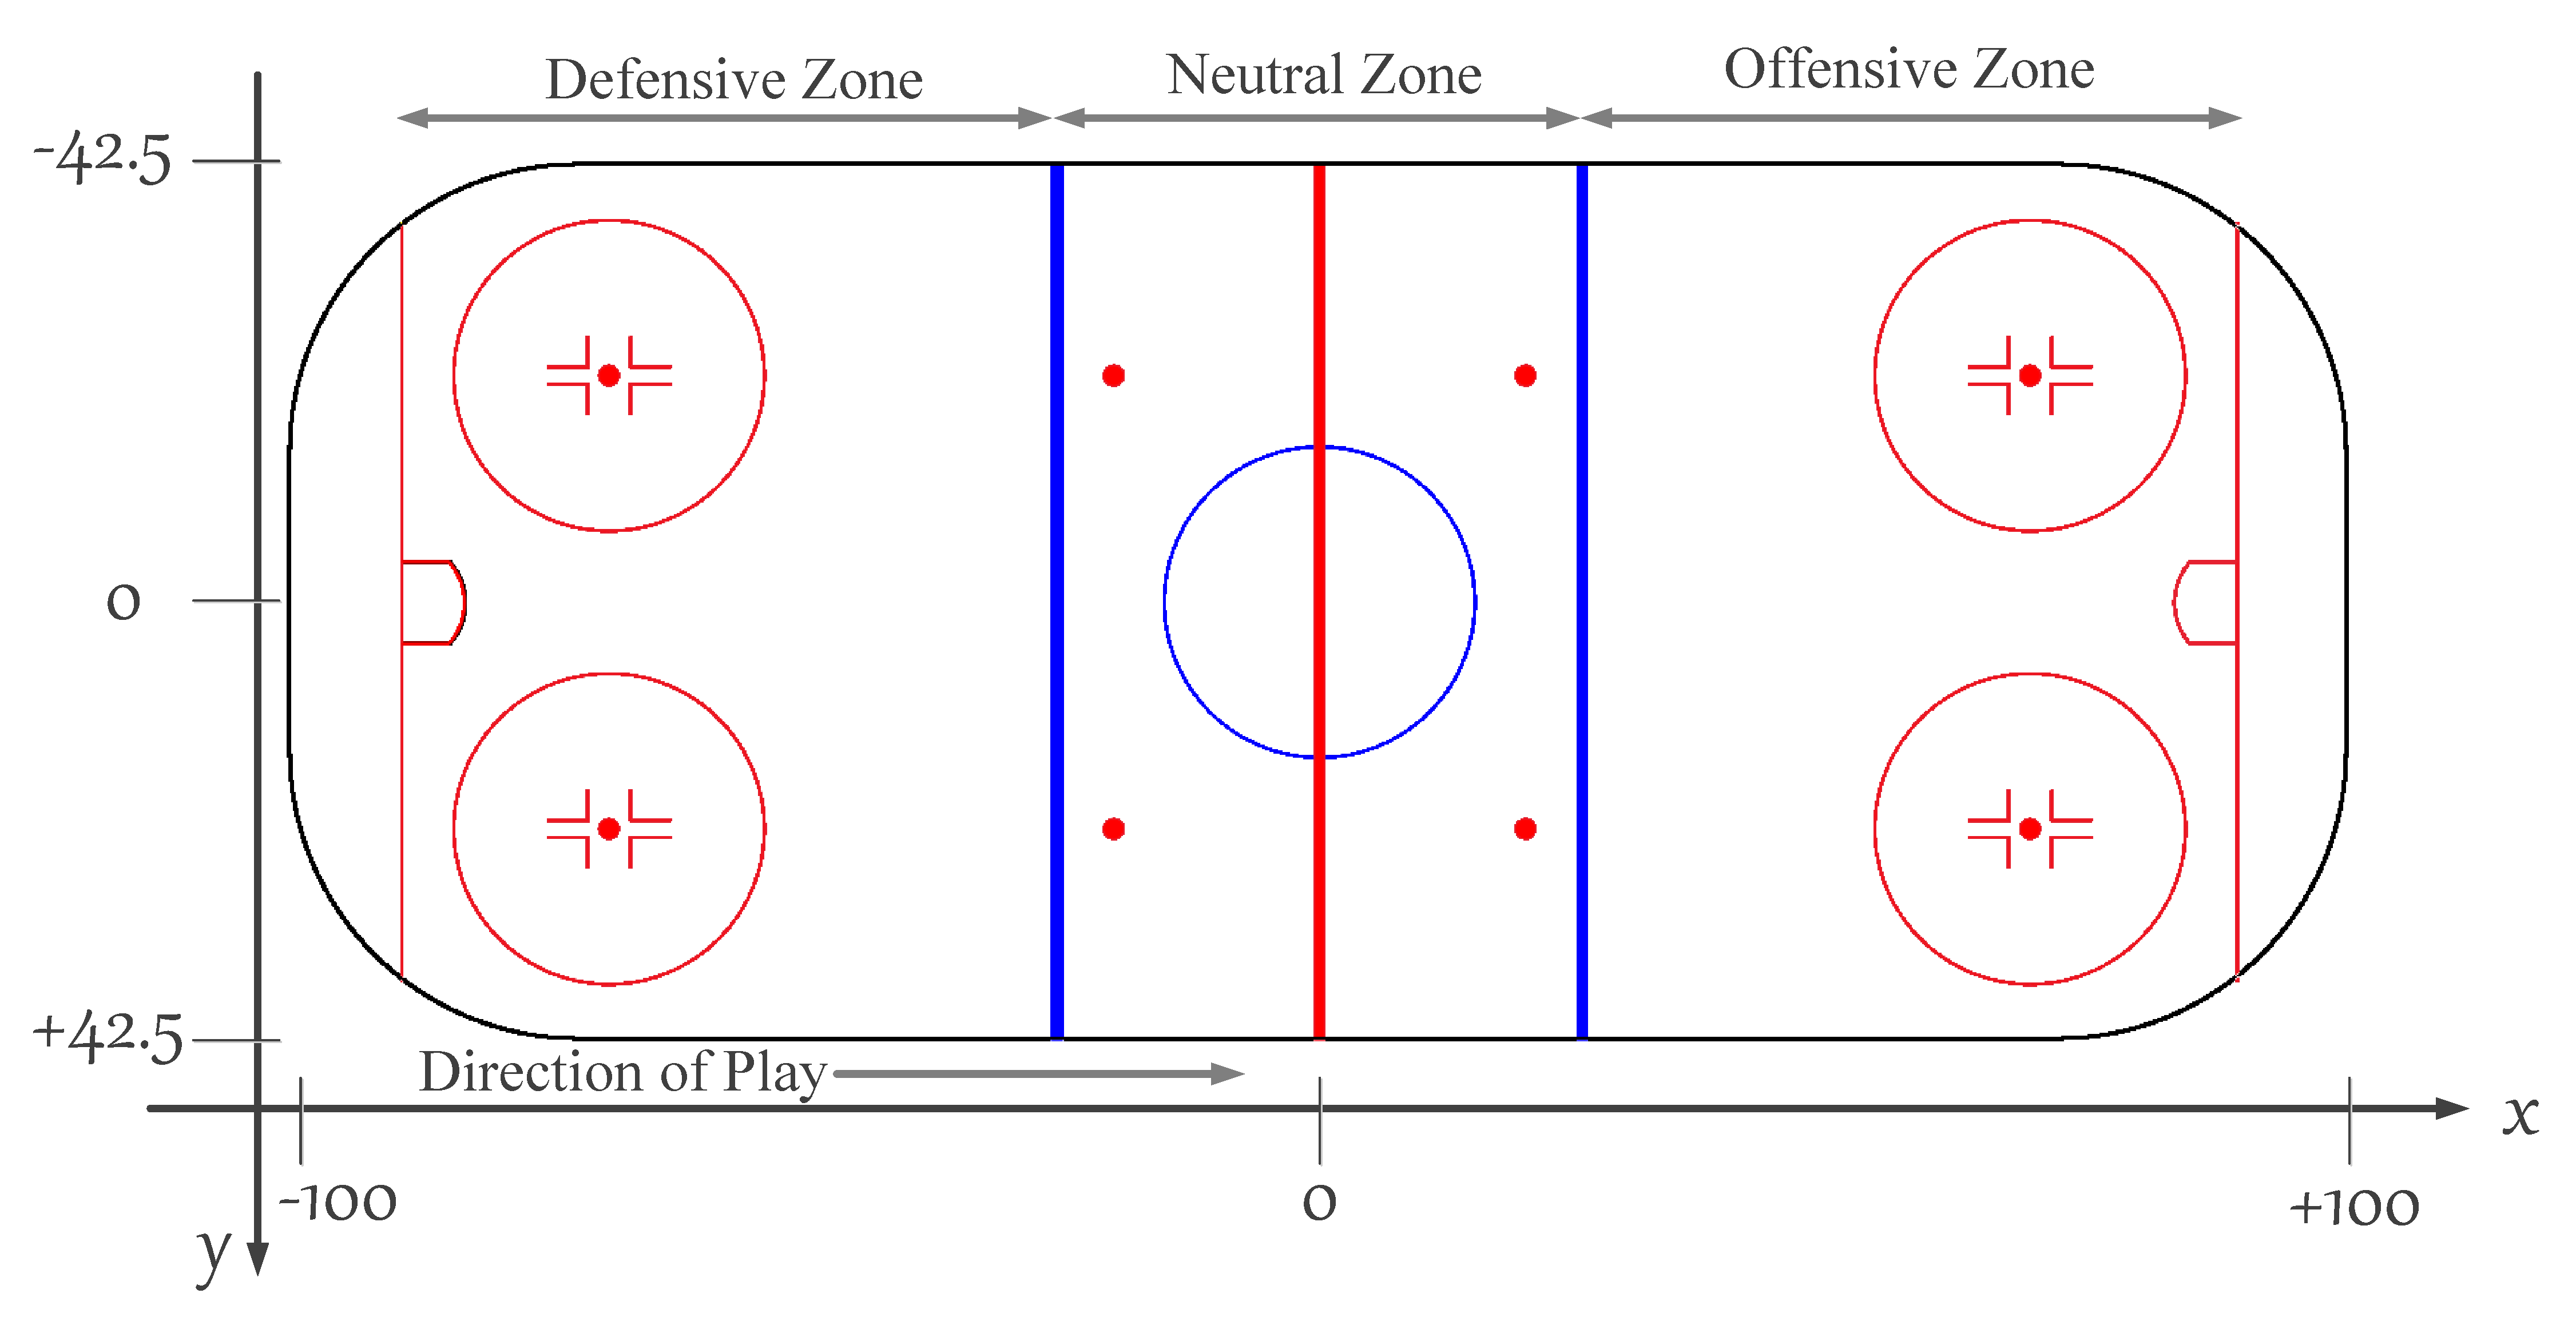
\includegraphics[width=1\textwidth]{rink}
		\caption{Rink Layout With Adjusted Coordinates. Coordinates are adjusted so that for the team performing an action, its offensive zone is on the right.}
		\label{fig:rink}
\end{figure*}

The clustering method we used was affinity propagation (AP) \citep{frey2007clustering}. AP is a clustering algorithm based on the idea of message passing between data points. It uses a set of real-valued pair-wise data point similarities as input.
  We used the negative of Euclidean distance between the data points as the measure of similarity. Unlike clustering algorithms such as k-means, AP does not need the number of clusters to be determined. AP automatically determines the number of clusters,
based on a preference hyperparameter $p(i)$; data points with higher preferences are more likely to be selected as cluster centers. The number of identified clusters can be increased or decreased by changing this value accordingly. A recommended default setting is to assign equal preference to all data points, and choose the shared preference value to be the median of the similarity values~\citep{frey2007clustering}. However, we found that this resulted in too many clusters to keep the Markov model state space tractable. We tried various multipliers, and found that setting $p$ to $4$ times the median of the similarity values for all data points led to a tractable number of clusters (typically 5, no more than 9 per action). 

For each action type, we found the set of $x$-$y$ points where the action type was performed, and we applied affinity propagation to produce a  custom clustering for the action type. This means that the locations maximize the information about where actions of the given type are performed.
Figure~\ref{fig:clustering} illustrates the resulting clusterings for shots and the two actions that occur most frequently in the SportLogiq dataset, passes (Figure~\ref{fig:pass}) and loose puck recoveries (Figure~\ref{fig:lpr}). The occurrence count is the number of times that the action is performed. We incorporated background knowledge by manually dividing the offensive zone into three clusters for shots (Figure~\ref{fig:shots}). Cluster 1 is an area known as the {\em slot}, Cluster 2 the area above and around the slot, Cluster 3 the area below and around the slot. In fact, affinity propagation discovered a similar clustering from the data.

\begin{figure}
		\centering     %%% not \center
		\subfigure[Clustering of Locations for Shots.]{\label{fig:shots}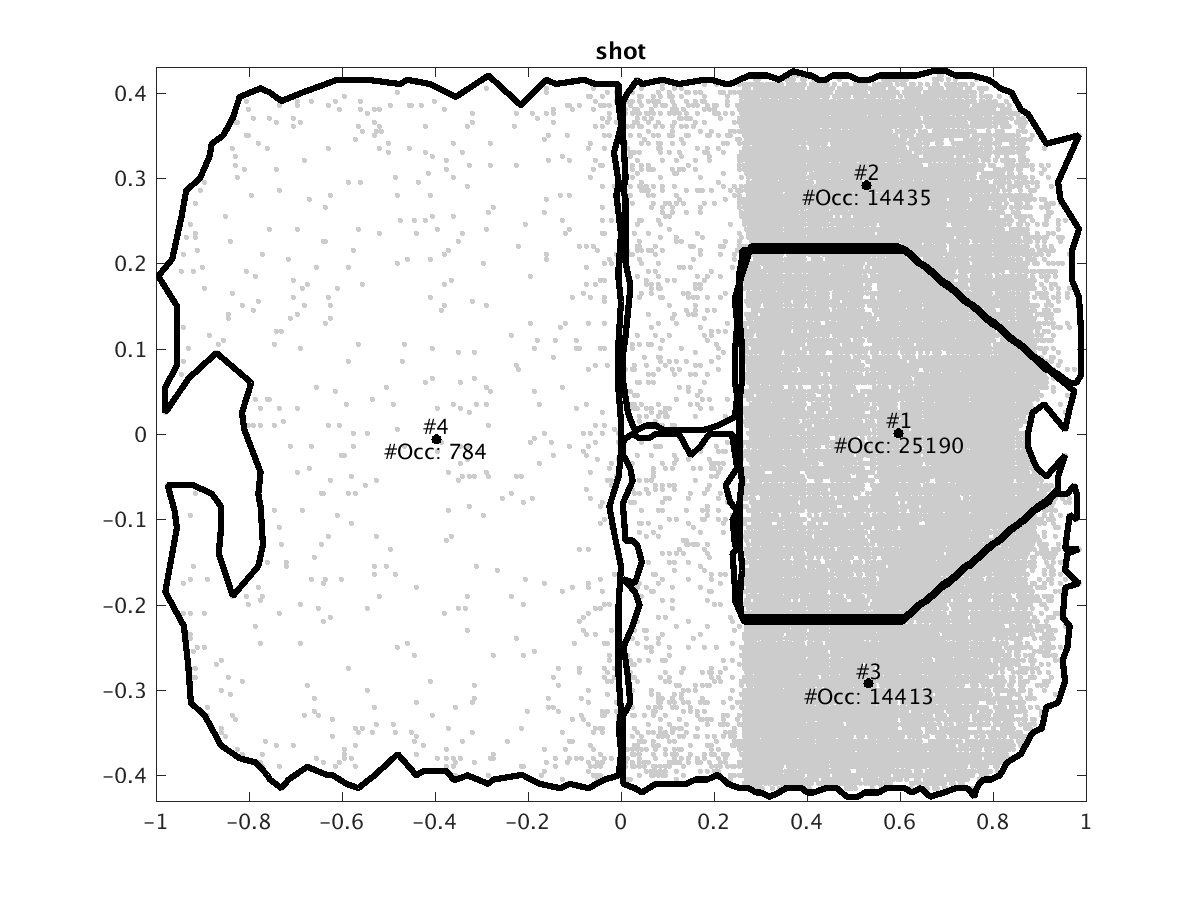
\includegraphics[width=0.8\textwidth]{shot}}
		\subfigure[Clustering of Locations for Pass]{\label{fig:pass}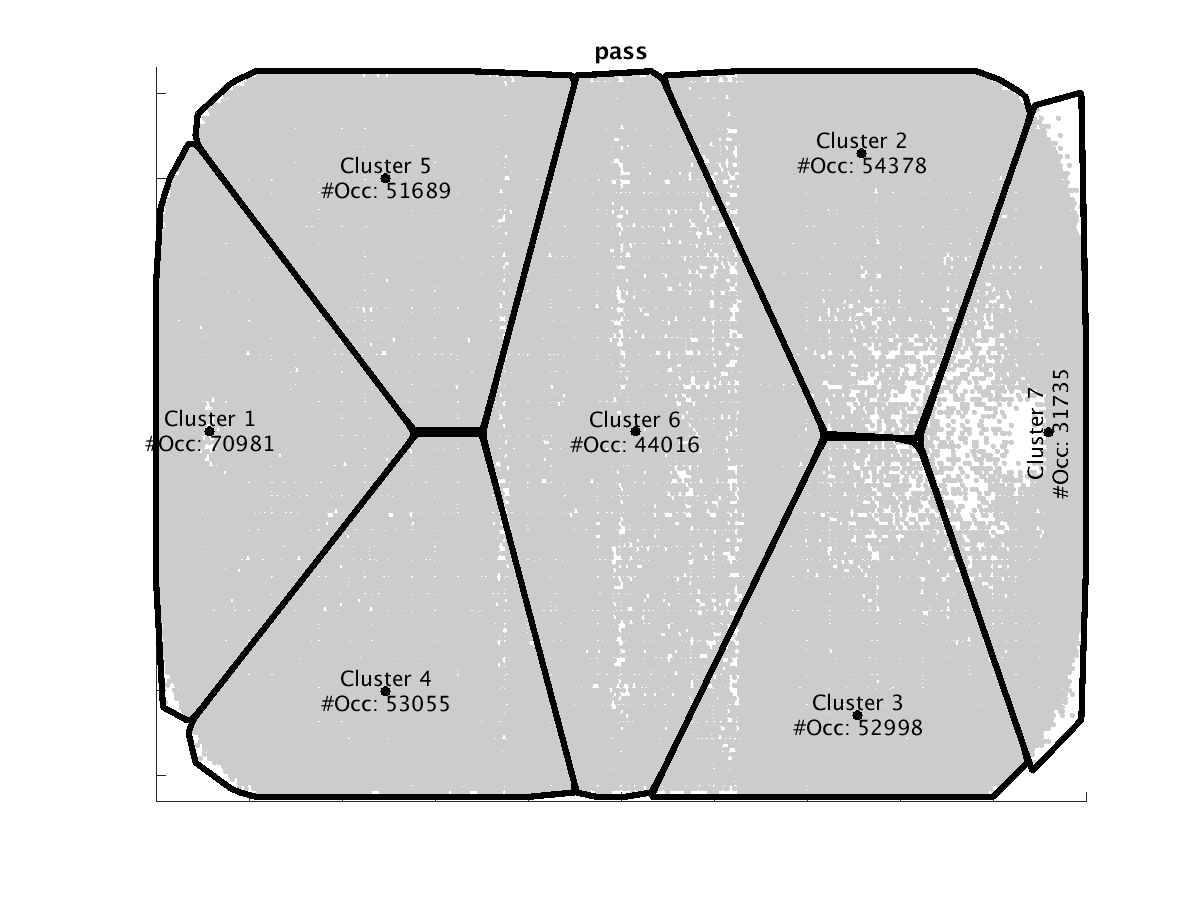
\includegraphics[width=0.8\textwidth]{pass}}
		\subfigure[Clustering of Locations for Loose Puck Recovery]{\label{fig:lpr}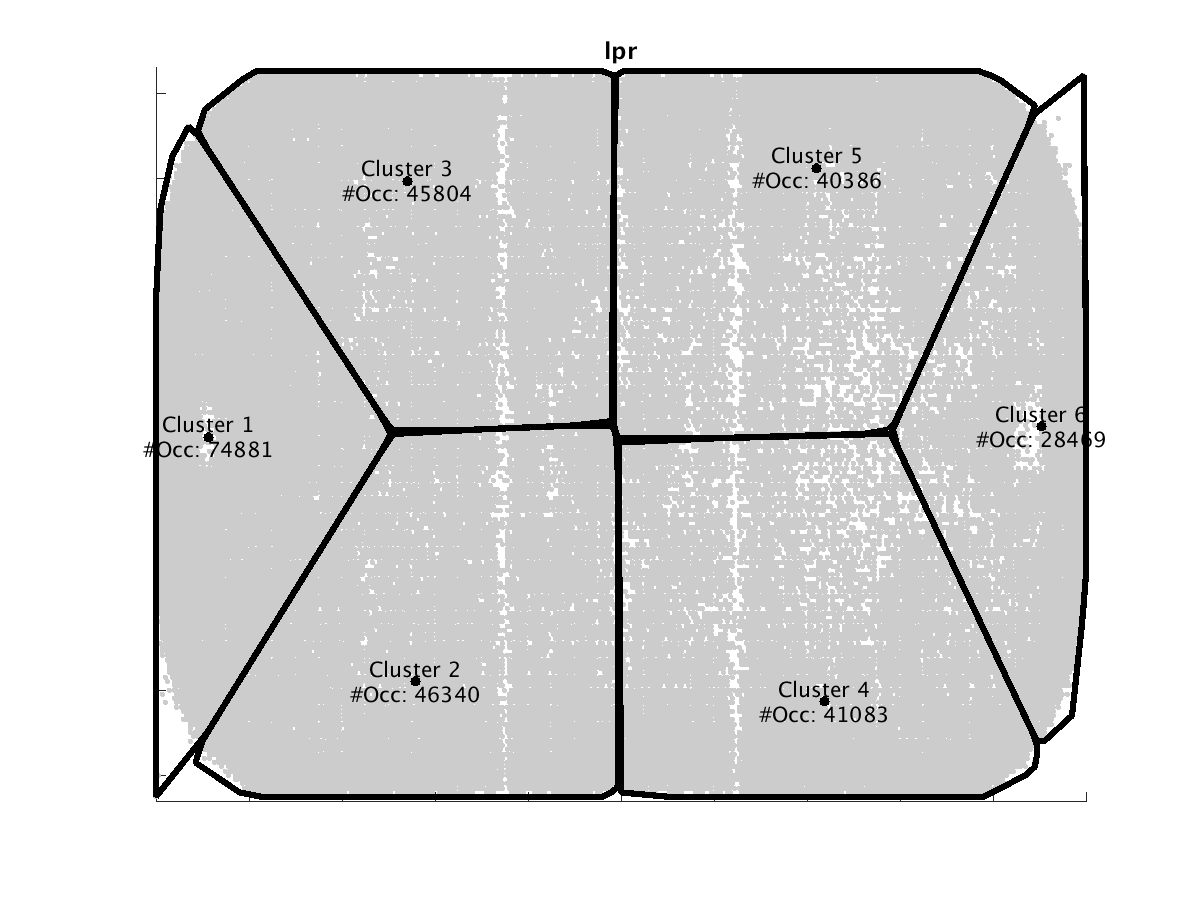
\includegraphics[width=0.8\textwidth]{lpr}}
		\caption{Locations are discretized separately for each action by clustering (affinity propagation). Gray dots indicate occurrences. The cluster mean is shown, with labels that indicate (i) the action occurrence count, (ii) the value of the action at different locations.}\label{fig:clustering}
	\end{figure}





\section{MARKOV GAMES}
A Markov Game \citep{Littman1994}, sometimes called a stochastic game, is defined by a set of states, $\mstates$, and a collection of action sets, one for each agent in the environment. State transitions are controlled by the current state and a list of actions, one action from each agent. For each agent, there is an associated reward function mapping a state transition to a reward. An overview of how our Markov Game model fills in this schema is as follows. There are two players, the Home Team $\home$ and the Away Team $\away$.
%The game is zero-sum, meaning whenever a home team receives a reward, the Away Team receives minus the reward. Therefore we can simply use a single reward value, where positive numbers denote a reward for the home team (the maximizer), and negative number a reward for the Away Team (the minimizer).
In each state, only one team performs an action, although not in a turn-based sequence.
This reflects the way the data record actions.
Thus at each state of the Markov Game, exactly one player chooses No-operation.
We introduce the following generic notation for all states, following \citep{Russell2010,Littman1994}.
%, and a modification of the notation used by \citep{Littman1994} is used to describe the multi-agent setup specific to NHL games. Notation for value iteration follows \citep{Mitchell1997}.

\begin{itemize}
\item $Occ(\mstate,\action)$ is the number of times that action $\action$ occurs in state $\mstate$ as observed in the play-by-play data.
\item $Occ(\mstate,\action,\mstate')$ is the number of occurrences of action $\action$ in state $\mstate$ being immediately followed by state $\mstate'$ as observed in the play-by-play data. $(\mstate,\mstate')$ forms an edge with label $\action$ in the transition graph of the Markov Game model.
\item The transition probability function $TP$ is a mapping of $\mstates \times \actions \times \mstates \rightarrow (0,1]$. We estimate it using the observed transition frequency $\cfrac{Occ(s,\action,s')}{Occ(s,\action)}$.
\end{itemize}

We begin by defining the state space, then the action space.


\subsection{STATE SPACE}
\label{subsec:context}

Previous work on Markov process models for ice hockey \citep{Thomas2013} defined states in terms of hand-selected features that are intuitively relevant for the game dynamics, such as the goal differential and penalties.
We refer to such features as \textbf{context features}. 
%The first way in which our model goes beyond such models is by including a larger set of context features. The second way is by including a history of actions as part of a state. This is a major extension in the level of modelling detail, but raises computational challenges in dealing with a much larger state space, which we address in this paper.

\begin{table}[htbp]
\caption{Context Features}
\label{table:context-features}
\begin{center}
%\resizebox{1\columnwidth}{!}{
%\begin{tabular}{|c|c|p{2cm}|c|}
\begin{tabular}{|c|c|c|}
%Notation & Name & Definition & Range \\\hline
%$\GD$ & Goal Differential & {Number Home Goals} - {Number Away Goals} & $ [-8,+8]$\\ \hline
%$\MD$ & Manpower Differential & {Number Home Skaters} - {Number Away Skaters} & [-3,3]\\ \hline
%$\period$ & Period & Current Period & [1,7]\\\hline
\hline
Notation & Name & Range \\\hline
$\GD$ & Goal Differential & [-8,8]\\ \hline
$\MD$ & Manpower Differential & \{EV,SH,PP\}\\ \hline
$\period$ & Period & [1,3]\\\hline
\end{tabular}
%}
\end{center}
\label{default}
\end{table}%

%\subsection{CONTEXT FEATURES}
A state lists the values of relevant features at a point in the game. These features are shown in Table~\ref{table:context-features}, together with the range of integer values observed.
Goal Differential $GD$ is calculated as Number of Home Goals - Number of Away Goals. A positive (negative) goal differential means the home team is leading (trailing).  Manpower Differential $MD$ specifies whether the teams are at even strength (EV), the acting team is short-handed (SH) or in a powerplay (PP).\footnote{Pulling the goalie can also result in a skater manpower advantage.} Period $P$ represents the current period number the play sequence occurs in, typically ranging in value from 1 to 5. Periods 1 to 3 are the regular play of an ice hockey game. Our model uses only periods from 1 to 3. Potentially, there are $(17 \times 3 \times 3) = 153$ context states. In our NHL dataset, $116$  context states occur at least once.



Most previous research on Markov process models of hockey has used only context features. A Markov process model with context features can answer questions such as how goal scoring or penalty rates depend on the game context \citep{Thomas2013}. However, it cannot answer questions about actions other than goals scored or penalties drawn. We next introduce the action space for our Markov game model that incorporates actions.


\subsection{ACTION SPACE}
\label{subsec:play-sequences}

The basic set of 13 action types was listed in Section~\ref{subsec:dataset}. Each of these action types has two parameters: which team $T$ performs the action and the location $L$ where the action takes place. We defined a discrete space of locations by discretizing continuous $x$-$y$ coordinates in a data-driven way; we present the details in Section~\ref{sec:locations} below. 
Using action description language notation \citep{bib:LevesquePirriReiter98}, we write action events in the form $\action(\team,\location)$. For example, $\it{block}(\it{Home},\location_{1})$ denotes that the home team blocks a shot at location 1. We usually omit the action parameters from generic notation and write $\action$ for a generic action event. There are 63 action-location pairs (sum of the number of clusters in table~\ref{table:eventsDef}), so considering we have two teams, home and away team, we have $63\times2 = 126$ possible action events that define transitions in the Markov game model. The total number of potential transitions is therefore $153\times126\times153 = 2,949,534$. The number of transitions we actually observe in the data is $112,590$. Our model assigns 0 probability to transitions that never occur, so the total number of parameters to estimate is $112,590$.


\subsection{REWARD FUNCTIONS}
\label{subsec:reward}

A strength of Markov Game modelling is that it can be applied with many reward functions, depending on what results are of interest ~\citep{Routley2015a}.
Our evaluation below utilizes two reward functions: 1) goal scoring, specifically scoring the next goal, and 2) winning. These can be defined as follows. 


\begin{enumerate}
\item For any state $\mstate$ where a Home resp. Away goal is scored, we set $\reward{\team}{\mstate}{\action} := 1$ where $\team = \home,\away$. For other states the reward is 0. 
%The \textbf{reward differential} is defined by $$\reward(\mstate,\action) := \reward_{\home}(\mstate,\action) - \reward_{\away}(\mstate,\action).$$
\item After a goal is scored, the next state is an absorbing state (no transitions from this state).
\item For any state $\mstate$ where the game ends with a win for Home resp. Away team, we set $\reward{\team}{\mstate}{\action} := 1$ where $\team = \home,\away$. For other states the reward is 0. All such states are absorbing states by definition.
%The \textbf{reward differential} is defined by $$\reward(\mstate,\action) := \reward_{\home}(\mstate,\action) - \reward_{\away}(\mstate,\action).$$
\end{enumerate}
%
%    \item $R_{\team}(s)$ is the reward value for each state $s$ received by team $\team$. This value depends on the objective being analyzed. $R_{\mstate} \equiv R_{\home}(\mstate)- R_{\away}(\mstate)$ is the reward differential, relative to the home team.
%\item Any $\mstate$ with a complete play sequence that ends in a Home resp. Away goal is an absorbing state (no transitions from this state).
%\item $Q_{\team}(\mstate)$ is the expected total reward obtained by a team, over all state sequences that start in state $\mstate$. $Q_{\mstate} \equiv Q_{\home}(\mstate)- Q_{\away}(\mstate)$ is \textbf{value} of state $\mstate$, relative to the home team.
%\item $Q_{i}(s)$ is the value iteration function value for state $s$ during iteration $i$. Note that $Q_{0}(s) = 0$ as an initialization step for the value iteration algorithm.

\subsection{STATE VALUES}

Given the specification of a Markov game model, 
the expected reward for a team %$Q_{\home}(\mstate)$
represents the expected total reward that a team obtains from a random walk through the state space of unbounded length. The expected reward from a starting state $\mstate$ is the \defterm{value} of a state, denoted $\evalue{\team}{\mstate}$ where $\team = \home,\away$. We will consider the expected total reward from random walks whose length is bounded by a constant $\lookahead$. The bound $\lookahead$ can be interpreted as the \defterm{look-ahead horizon}.  Strictly speaking, the value of a state depends on the transition probabilities, and on the look-ahead horizon. These will be implicitly fixed by context, so we do not  show the dependency explicitly in our value function notation. For a given reward function, we learn an appropriate look-ahead horizon from the data  (see Section~\ref{subsec:value-iteration-alg} below). 

We also consider the \defterm{conditional state value}. The conditional value for the home team is the value for the home team performing an action, divided by the sum of the value for the home team and the value for the away team. Similarly for the away team. The conditional value corresponds to conditioning on the event that at least one of the team scores a goal within the next 14 time steps (our look-ahead horizon). It measures the expected reward of a team relative to its opponents, in other words, the advantage that a team enjoys over its opponent in a given match state. For example, with reward = scoring the next goal, a conditional value of $p$ for the home team means that, given that one of the teams will score the next goal within the look-ahead horizon, the chance is $p$ that the home team manages the next goal.

\paragraph{Discussion} Winning the game is the ultimate aim of a team. \citep{Pettigrew2015} estimates a Markov model value function with winning as reward function. With winning as the reward function, the value of a state for a team is the chance that the team wins the game if play starts from that state (within the look-ahead horizon).

Goals are the events with the most impact on winning chances. With scoring the next goal as the reward function, the  value of a state for a team is the chance that the team scores the next goal (within the look-ahead horizon). This value function generalizes action values used previously in hockey analytics, such as Expected Goals (from a shot) \citep{Tegen2015,Graphs2015}. It is also comparable to the expected possession value (EPV) that  \citep{Cervone2014a} define for their basketball Markov model, in that both measure the expected score in the current local play, rather than the global chance of winning the game overall.
%The next goal objective can be represented in the Markov Game model as follows.


 
%The reward differential is the difference in these probabilities. It is consistent with the practice in zero-sum game theory of assigning a single value to a game outcome: +1 for the maximizer, -1 for the minimizer, 0 for a tie~\citep{Russell2010}. 
%
%In a single-agent setting with a fixed policy, the value of a state is the expected reward for following the policy from the state. In the game-theoretic setting with two agents, we need to consider the difference in rewards. In a zero-sum game, the value of a state is the final result following optimal play. Intuitively, the value specifies which player has a better position in a state. Since we are not modelling optimal play, but actual play in a policy-on setting, the expected difference in rewards is the natural counterpart. We define the total reward over a state sequence as the sum of rewards, and while typically computed with a discount factor, discounting or averaging is not natural in ice hockey. For example, winning the game has the same value for a team regardless of how many actions occurred previously. Goals may be more valuable if they are scored after fewer actions, but this should be an empirical finding from the analysis, not built into the definition of the reward function. As such, we do not discount, following \citep{Schwartz1993}. Using undiscounted rewards raises issues about the convergence of an infinite sum of rewards. We discuss these below in connection with the value iteration algorithm.





\section{DYNAMIC PROGRAMMING}
\label{subsec:value-iteration-alg}

We describe an algorithm for computing the value of a state. If each state appeared at most once between goals, we could compute the Next Goal value function for, say the home team, simply as follows: count the number of state occurrences that were followed by a home goal, and divide by the total number of all state occurrences. However, a state may appear any number of times between goals. That is, the transition graph may contain loops. In that case the value function can be computed by an iterative procedure known as dynamic programming (DP). The key observation is that any value function satisfies the {\em Bellman equation}:

\begin{equation} \label{eq:bellman}
\evalue{\team}{\mstate} =  \sum_{\mstate',\action} P(\mstate,\action,\mstate') \times \evalue{\team}{\mstate'}
\end{equation}

where $\team = \home,\away$. Value iteration starts from an initial value assignment---typically 0 for each state---then applies the Bellman equation as an update equation. We compute the state values for both home and away teams. The iteration stops when the change in state value differential between the home and the away team falls below a convergence threshold. In our experiments, we use a relative convergence of 0.1\% as the convergence threshold. Algorithm~\ref{alg:value-iteration-dynamic} provides pseudo code. 




\begin{algorithm}
\caption{Dynamic Programming for State Value Computation, for the reward differential function $R$.}
\label{alg:value-iteration-dynamic}
\begin{algorithmic}[1]
\REQUIRE Markov Game model, convergence criterion $c$
 \STATE{$InitialValue = 0$}
\FOR{$\lookahead = 1; \lookahead \gets \lookahead + 1$}
    \FORALL{states $s$ in the Markov Game model}
    \FORALL{teams $\team = \home,\away$}
    
            \STATE{$ V_{\team}^{\lookahead+1}(\mstate)$ := \\ $\sum_{\action} \reward{\team}{\mstate}{\action} + \sum_{\mstate'}\cfrac{Occ(s,\action,s')}{Occ(s,\action)}\times V_{\team}^{\lookahead}(s')$}

    \ENDFOR
    \ENDFOR
 \IF{$|[V_{\home}^{\lookahead+1}(\mstate) - V_\team^{\lookahead+1}(\mstate)]-[V_{\home}^{\lookahead}(\mstate) - V_\team^{\lookahead}(\mstate)]| < c$ for all states $\mstate$}
 \STATE{EXIT}
 \ENDIF
%    \STATE{$lastValue = currentValue$}
%    \STATE{$currentValue = 0$}
\ENDFOR
\end{algorithmic}
\end{algorithm}

\paragraph{Discussion} We use an undiscounted reward function for our value iteration \citep{Schwartz1993}. 
%This means that as the look-ahead horizon $\lookahead$ increases, the expected reward for a single team increases without convergence, because a longer random walk has a higher chance of reaching a goal state. However, with a sufficiently look-ahead from the initial state, the additional expected reward from taking another step becomes essentially the same for both the home and the away team. Therefore our convergence test looks at the temporal difference of the simultaneous value differences between the home and the away team. 
In game terms, the convergence criterion can be interpreted as follows. The quantity $V_{\home}^{\lookahead}(\mstate) - V_\team^{\lookahead}(\mstate)$ measures the home team advantage in state $\mstate$, given a look-ahead horizon $\lookahead$. (A negative advantage represents a disadvantage.) We stop value iteration when the algorithm's estimation of the home team advantage has converged, relative to our tolerance. This is appropriate for a zero-sum game because the aim of the game is to achieve an advantage over the opponent.


 With this convergence criterion, DP converges within 14 steps for the Next Goal reward function. This means that looking ahead more than 14 steps changes the estimate of the how much more likely the home team is to score the next goal than the away team,  by less than 0.1\%. For the Win reward function, convergence requires 1,950 iterations until the win probability differential falls below 0.1\%. This is because the algorithm looks ahead to the complete end of the game rather than just to the next goal.
%



%Make sure all notation is defined.

%\subsection{CONVERGENCE} %Discuss convergence.
%
%Each iteration $i$ of the dynamic programming algorithm computes the value of a state with a look-ahead window of at most $i$ steps. As the limit of $i$ goes to infinity, each path of at most $i$ steps from a state will either end in the objective event, such as a goal, or the end of the match. The occurrences of the end of match are much smaller than the number of goals or penalties, so approximately every path will end with the objective event for either the home team or the away team. As such, the value of each state will converge to the conditional probability of the home or away team's objective event. As we use rewards with bounded sums, the computations of expected values also converge by extension.

%\subsection{EXAMPLE}
%
%We will first give a small example of the context-inclusive Markov Decision Process construction. This will be followed by a few iterations of the value iteration dynamic programming algorithm.


%Readers love examples, stepping through a computation is fine.

%\subsection{THEORETICAL JUSTIFICATION}

%Sometimes this comes first, for instance if your algorithm is based on a mathematical derivation. You could also at this point include a correctness proof, or a complexity analysis (e.g., theoretical upper bound on run-time).

%\subsection{DISCUSSION}

%The context state space consists of goal differential, manpower differential, and period as context variables. Goal differential, manpower differential, and period typically remain fixed during a play sequence. The exception to this rule is that manpower differential can change during a play sequence when the goalie is pulled or a penalized player returns to the ice. The zone was left out context state space in order to decrease the number of context subtrees, which also reduces the number of nodes. Instead, zone is included in the action-event. %The change in the number of states with and without manpower differential is observed in Table~\ref{table:size-of-mdp}.

%There may be a need for discussion, for instance why you made certain design choices or how your algorithm is different from that used by others.


\section{EXAMPLES} 
We provide some examples of how our Markov game model evaluates actions in context. This illustrates our results for the hockey domain. For readers less familiar with dynamic models, the examples illustrate the concept of look-ahead.

\subsection{High-Value Trajectory through the State Space} 

The model can be used for a planning task: to  find successor states that are most likely to lead to a goal. Figure~\ref{fig:trajectory} shows a high-value trajectory where a state is connected to its highest value successor (for the Home team). 

\begin{figure*}
\centering 
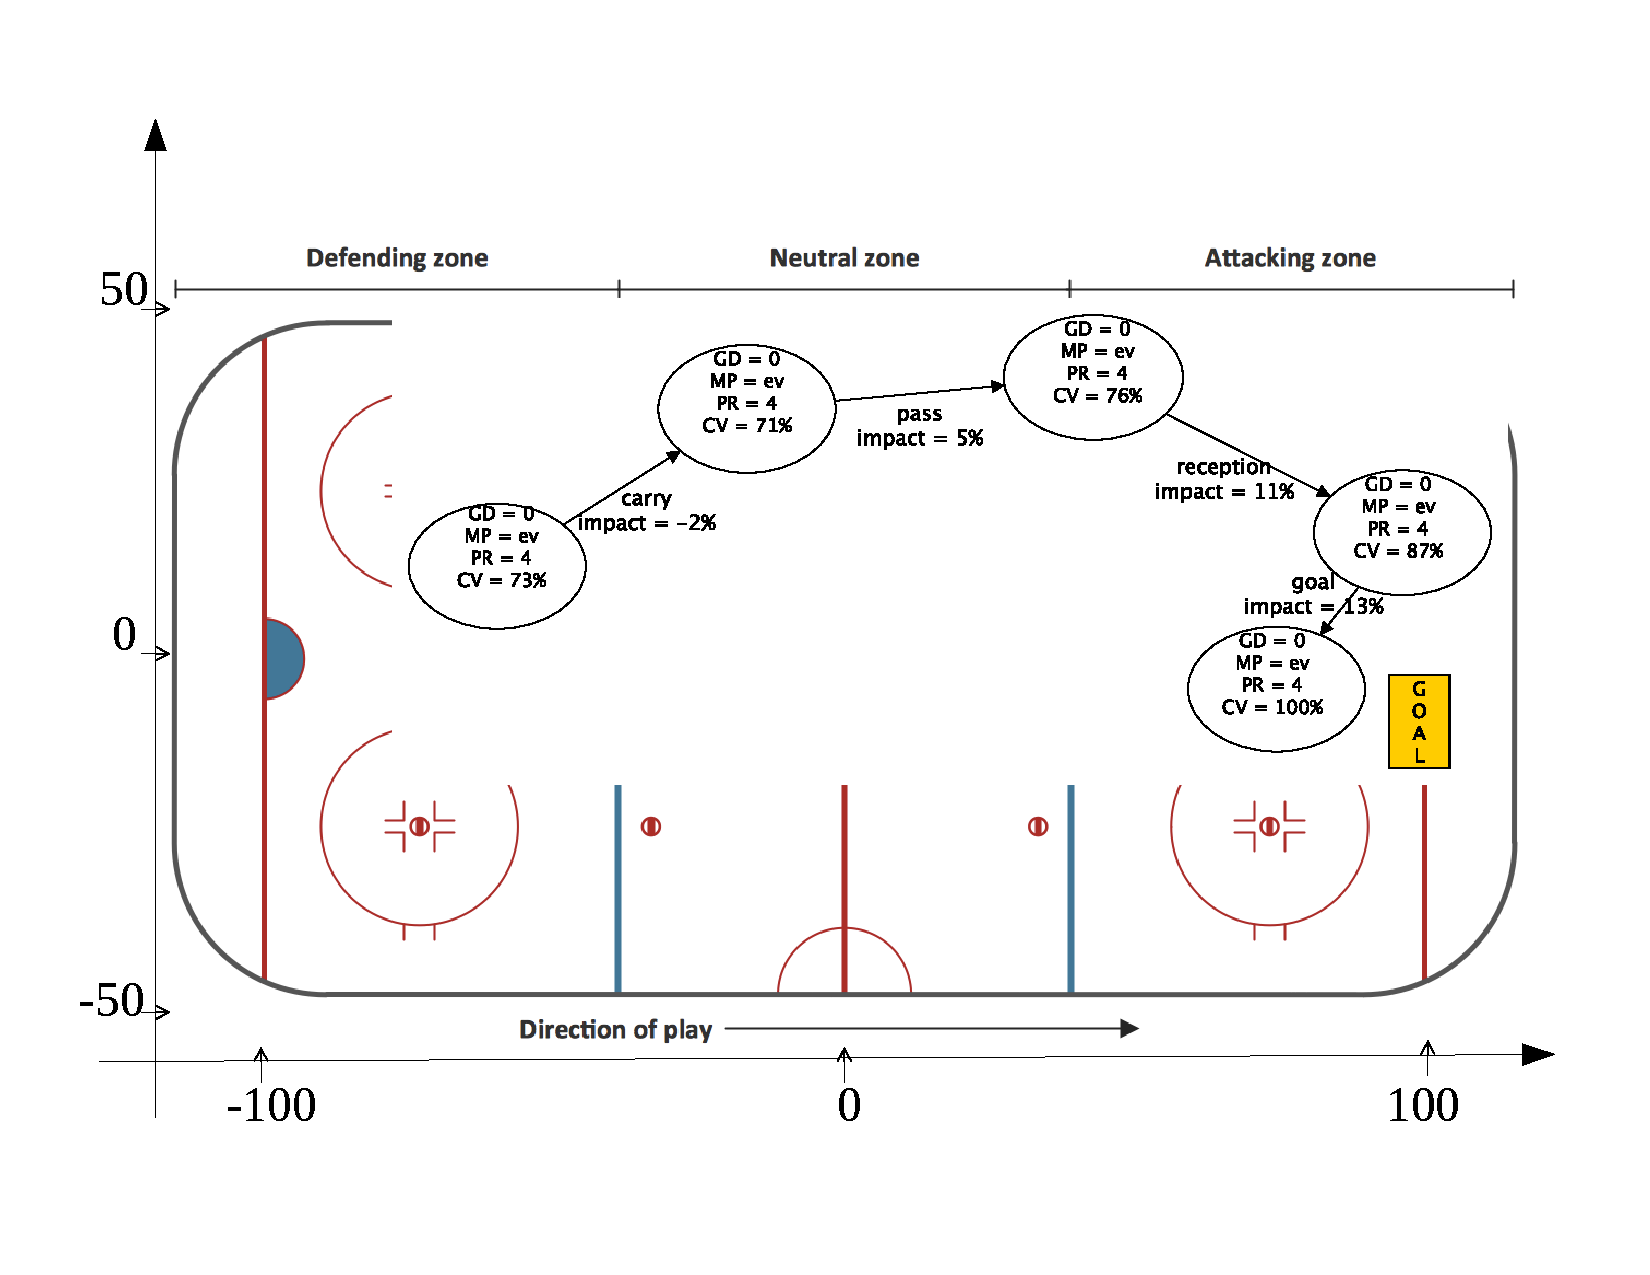
\includegraphics[width=1\textwidth]{trajectory-rink}
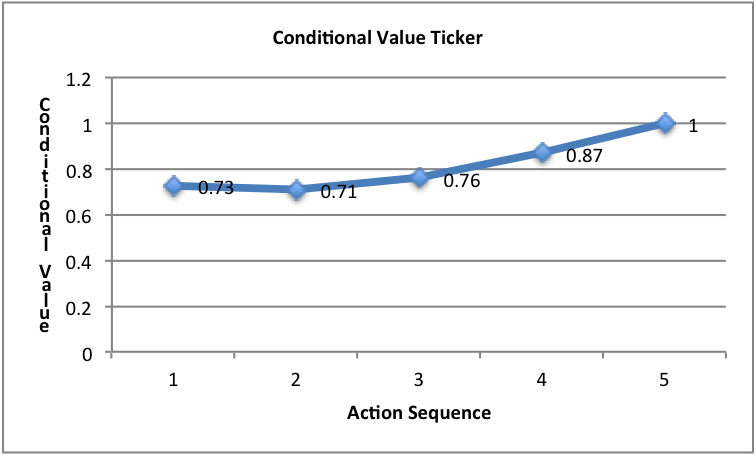
\includegraphics[width=0.9\textwidth]{value-ticker.png}
\caption{A high-value trajectory that represents one generic successful play by the home team. {\em Top:} We show a rink outline for orientation. Location coordinates are rescaled to bring nodes closer for legibility. A node represents a game state. Nodes are labelled as follows. GD = goal difference. MP = manpower, PR = period. CV = conditional value of a state for the home team (= probability that the home team scores the next goal, see below). Edges are labelled with actions, and with the impact of the action, which is the difference in conditional probabilities (see Section~\ref{sec:perform}). {\em Bottom:} The same trajectory using a value-ticker format \citep{Cervone2014a}, where the conditional value of the current state is  plotted against events in temporal sequence. The horizontal distance between points is the impact of the corresponding action. }
\label{fig:trajectory}
\end{figure*}



\subsection{Action Values}

We can evaluate an action in a context-aware way by considering its expected reward after executing it in a given state. This is known in reinforcement learning as the action value, or \textbf{Q-value}~\citep{bib:sutton}:

\begin{equation} \label{eq:q-value}
Q_{\team}(\mstate,\action) \equiv \sum_{\mstate'} P(\mstate,\action,\mstate') \times \evalue{\team}{\mstate}
\end{equation}

where $\team = \home,\away$.
As with state values, we can also consider \defterm{conditional Q-values}. The conditional Q-value for the home team is the Q-value for the home team performing an action, divided by the sum of the Q-value for the home team and the Q-value for the away team. Similarly for the away team. 
%The conditional Q-value corresponds to conditioning on the event that at least one of the team scores a goal within the next 14 time steps (our look-ahead horizon). It measures the expected reward of a team relative to its opponents, in other words, the advantage that a team enjoys over its opponent in a given match state. For example, with reward = scoring the next goal, a conditional Q-value of $p$ for the home team means that, given that one of the teams will score the next goal within the next 14 time steps, the chance is $p$ that the home team manages the next goal.

To obtain a single value of an action at a location, we average over some or all of the context features.  For example, to evaluate the chance of scoring from a shot location, we average over all shots at that location in all periods, and at all manpower levels. In the following we provide 2D gray scale plots of the value surface for a given location. The $x$-$y$ coordinates in these plots are {\em adjusted coordinates}, so the defense zone locations are assigned negative $x$-values. 
%The 3D plots are best viewed on screen for color.

\subsubsection{Shots}

Figure~\ref{fig:shot-values} shows the values of shots from different locations, with look-ahead $\lookahead = 1$, i.e., considering immediately following goals only, and $\lookahead = 14$, our maximum look-ahead.

\begin{figure*}
\centering 
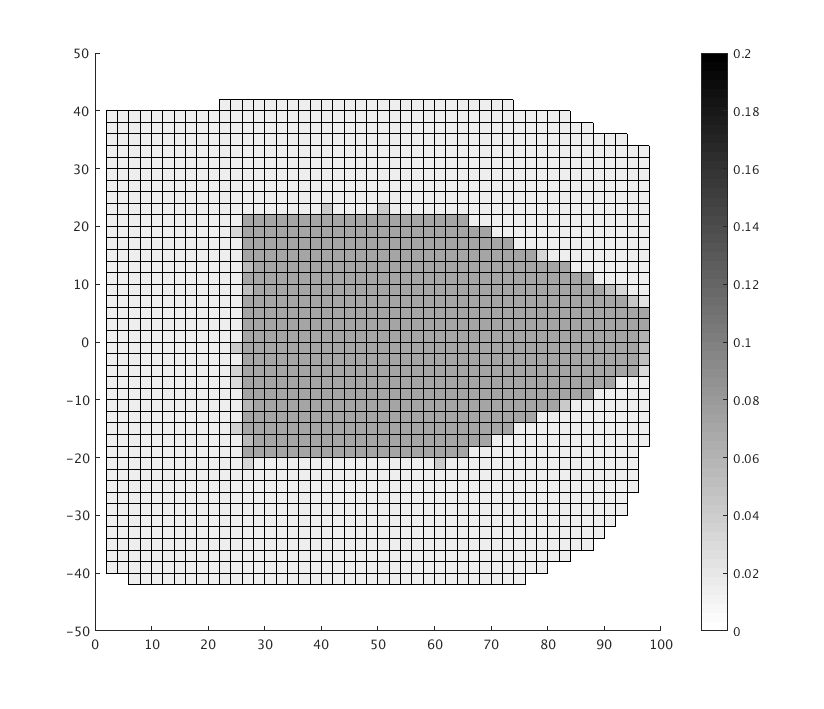
\includegraphics[width=0.48\textwidth]{shot2d.png}
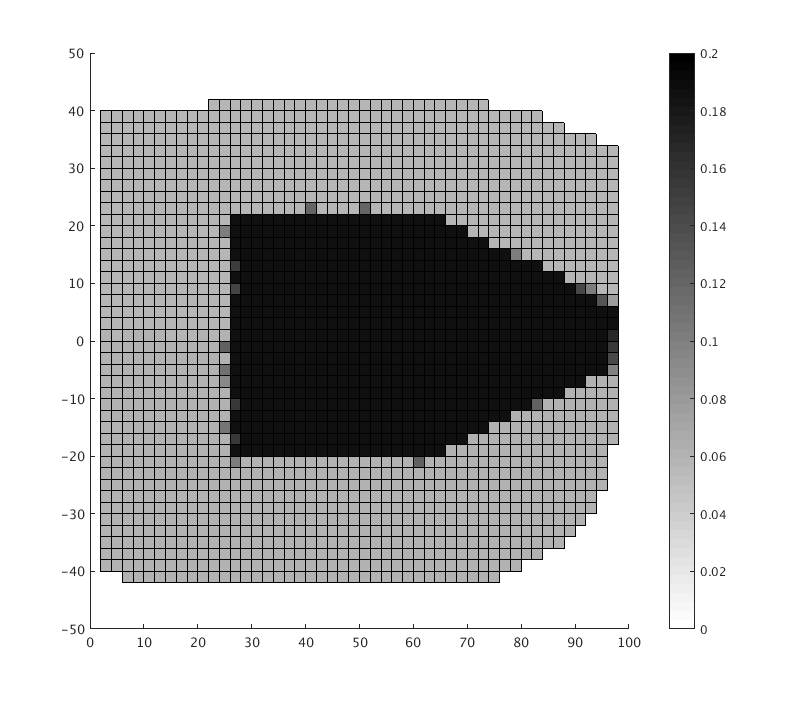
\includegraphics[width=0.48\textwidth]{shotvalue3d.png}
\caption{Average values of shots depending on location. The value indicates the probability that a shot will be followed by a goal within look-ahead $\lookahead = 1$ or 14 steps. It is averaged over the context features (goal differential, manpower, period) and the shooting team (Home or Away). Locations in the same cluster are treated as equivalent by the Markov game model, and therefore are assigned the same value. Left: The highest chance of scoring immediately on a shot is from the slot (6\%). The clusters around the slot carry a chance of about 1.5\%. Right: The chance of scoring after a shot within our look-ahead horizon of 14 steps. This includes immediate goals as well as rebounds. The medium-term probability is greater, around 16\% for shots from the slot, and around 6\% for the other clusters.}
\label{fig:shot-values}
\end{figure*}

\subsubsection{Loose Puck Recoveries} 

Figure~\ref{fig:lpr-values} shows the average location values for {\em loose puck recoveries.} Loose puck recovery is a frequent event in the Sportlogiq dataset. It is an interesting event to consider, because it is fairly neutral with respect to goal scoring, so approaches that consider immediate goal consequences only find it difficult to assign a value to it. In our model, with look-ahead $\lookahead = 1$, the expected reward from loose puck recovery vanishes almost everywhere; see Figure~\ref{fig:lpr-values}(top right). (Zero except for two clusters with value 0.0002 and 0.0001.) Figure~\ref{fig:lpr-values}(left) shows that with look-ahead $\lookahead = 14$, there is considerable variation in the values for different location. We see how the action value changes depending on whether the defending or the attacking team recovers the loose puck: The conditional chance of scoring the next goal for the attacking team is around 73\% in the right bottom of the offensive zone (Cluster 4 in Figure~\ref{fig:lpr}). For the defending team, in the same physical location, it is around 53\%. So by beating the attacking team to a loose puck recovery, the defending team increases its chance of scoring the next goal by 20\%.  This illustrates an important way in which the model captures the value of defensive actions: The chance that the defending team scores the next goal increases by decreasing the chance that the attacking team scores the next goal. 

\begin{figure*}
\centering 
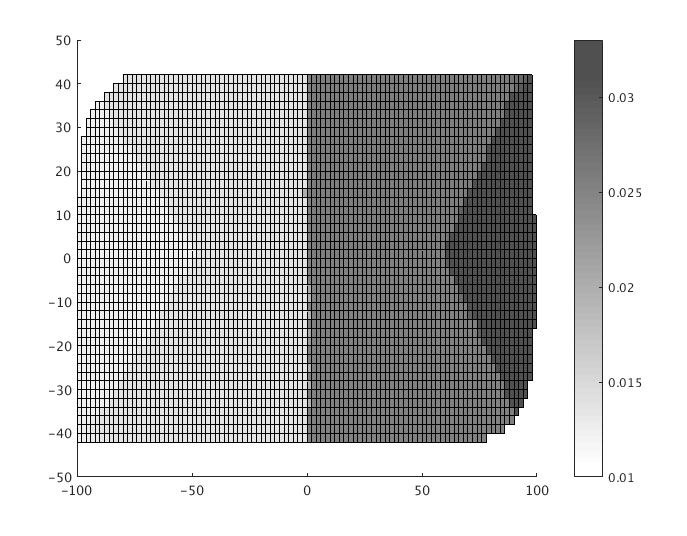
\includegraphics[width=0.48\textwidth]{lpr2d.png}
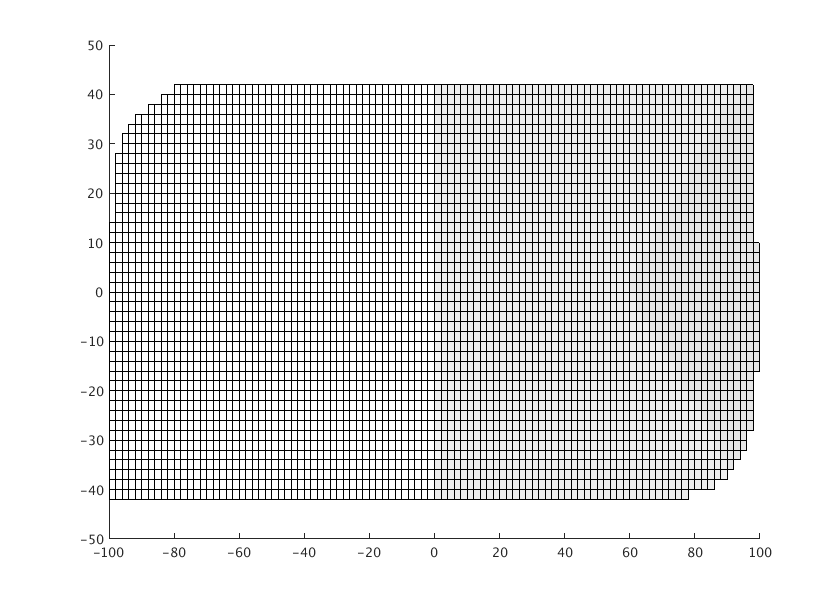
\includegraphics[width=0.48\textwidth]{lpr2dL1}
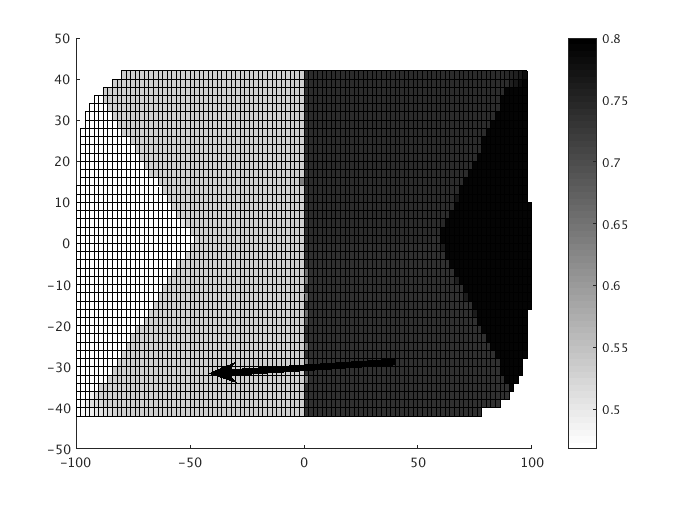
\includegraphics[width=0.48\textwidth]{lpr-match}
\caption{Left: Average value of loose puck recovery depending on location with look-ahead $\lookahead=14$. Right: Average value of loose puck recovery depending on location with $\lookahead=1$. Bottom: Average {\em conditional} value of loose puck recovery depending on location with $\lookahead=14$. The arrow connects the centre of Cluster 4 with the centre of Cluster 2. Using adjusted coordinates, it connects the same physical $x$-$y$ location, but with different values depending on whether the defending team or the attacking team manages the loose puck recovery.}
\label{fig:lpr-values}
\end{figure*}

\subsubsection{Dumping In the Puck vs. Carrying the Puck} 

Figure~\ref{fig:dumpin} shows two important offensive strategies: dumping the puck in (towards the goal) vs. carrying it (towards the goal).  

\begin{figure}
\centering 
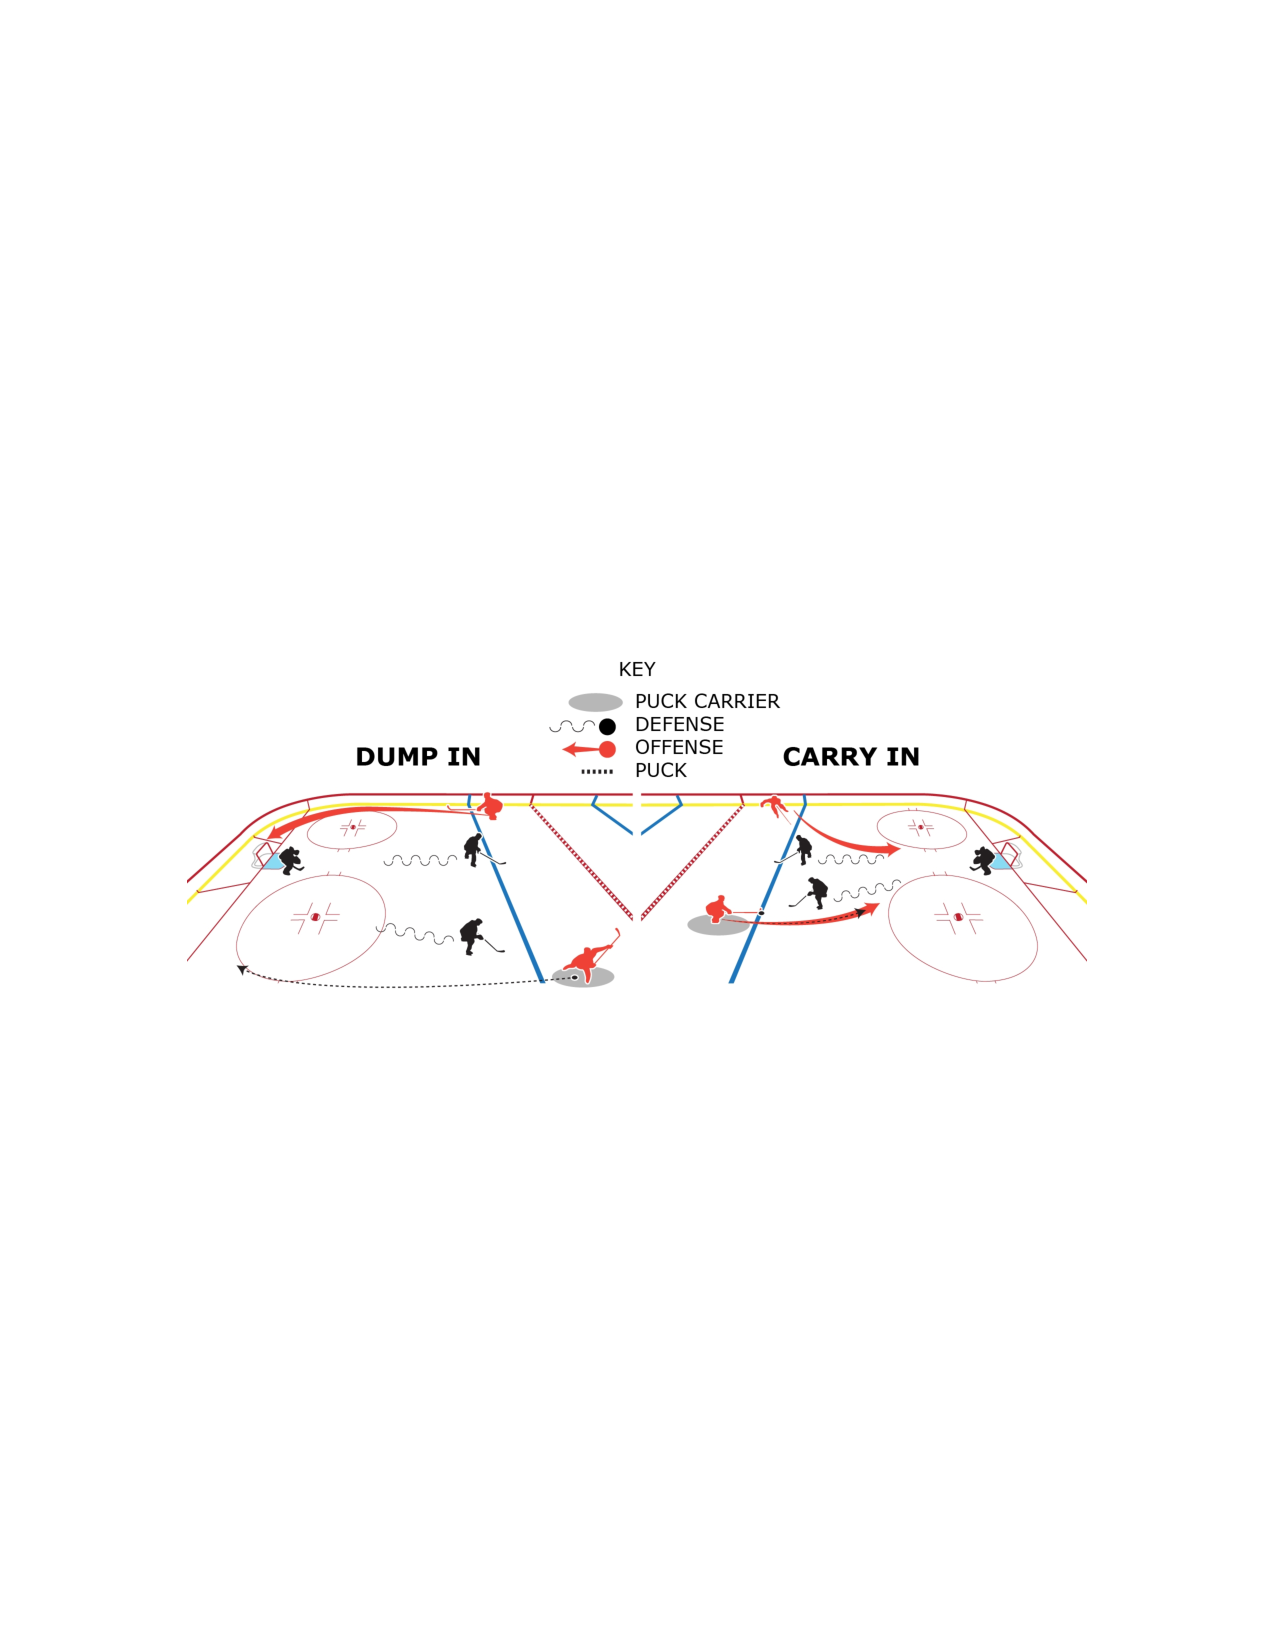
\includegraphics[width=1\textwidth]
{dumpvscarry}
\caption{Getting Into the Offensive Zone: Dumping vs. Carrying the Puck. Image by Shaun Kreider, Kreider Designs.}
\label{fig:dumpin}
\end{figure}


The comparative merits of each strategy are debated by hockey analysts \citep{Tulsky2013a}. Although these are two different actions, the expected reward provides a common scale on which they can be meaningfully compared; see Figure~\ref{fig:dump-values}. Generally carrying is more likely to lead to a successful attack: the conditional value for carrying ranges from 64\% to 76\%, whereas for dumping the puck it is fairly constant around 56\%. This agrees qualitatively with previous analyses that observe a higher correlation between carrying and success than between dumping in and success \citep{Tulsky2013a}. Some analysts conclude that players are too conservative: they prefer dumping in the puck towards the goal, rather than carrying it and losing possession. 
%However, we observe that the puck tends to be carried closer towards the opponent's goal.\footnote{need to check coordinates: Carrys are marked on the blue line. Clearer discussion of the clusters, visualizing them as well. Need to discuss zone-by-zone, dumps vs. carries.} For example, the adjusted $x$-coordinates of the cluster means for Carry are 0.02, 24.88, 24.8, 22.05, whereas for Dump In they are 5.96, 6.08, 5.67. 
Another hypothesis is that players carry the puck when the opposing defence-men are not well positioned to stop them. Investigating this hypothesis requires tracking data that record the position of all players at a given point.
%when players have the puck further away from the goal, they do not carry it because the risk of losing the puck to a challenge is too great when there is a long distance to go. They may therefore choose to dump or to carry appropriately in reaction to their current location. This analysis is an example of the considerations that are made possible by location data, and by considering the context of an action.  

\begin{figure*}
\centering 
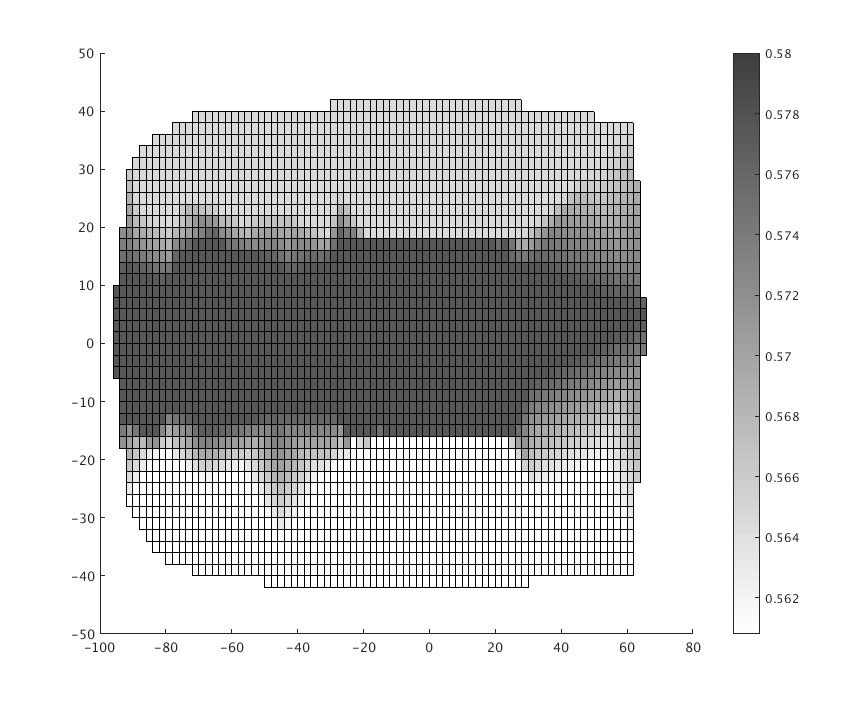
\includegraphics[width=0.48\textwidth]{dumpinCond2d.png}
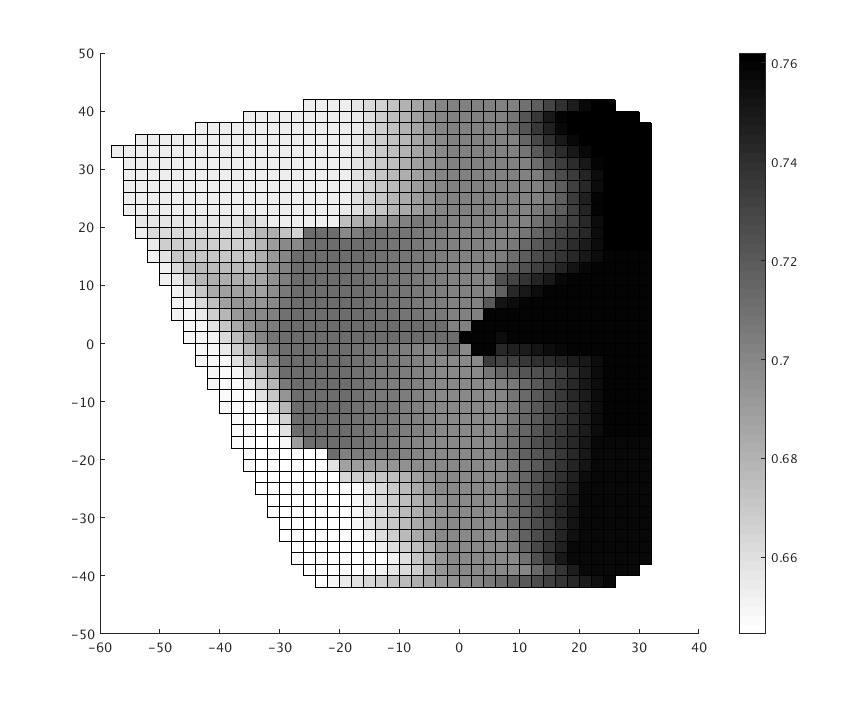
\includegraphics[width=0.48\textwidth]{carryCond2d.png}
\caption{Average conditional value of dumping in the puck (left) vs. carrying it (right).}
\label{fig:dump-values}
\end{figure*}


\section{TEAM PERFORMANCE}
\label{sec:perform}
We validate our model by showing that it can be used to evaluate team performance. We examine two approaches, first, team performance as an aggregate of action values, and second, team performance as an aggregate of state values.

\subsection{Team Performance and Action Values}
The general idea is that team strength can be estimated as an aggregate of individual action values, and then correlated with ground truth metrics such as numbers of goals scored. For example, the Expected Goal metric scores each shot according to its chance of leading to a goal (immediately)~\citep{Tegen2015}. The sum of goal probabilities for each shot is the team's Expected Goal metric. This metric was recently used by the Financial Times to analyse the reasons for Jose Mourinho's departure from the Chelsea Premier League team. The Expected Goal metric is a special case of our value function, where look-ahead $\lookahead = 1$ and the only action type taken into consideration is a shot. 

Schulte and Routley used the \textbf{goal impact metric} to rank players~\citep{Routley2015a}. The impact of an action is defined by the equation

\begin{equation}
\impact_{\team}(\mstate,\action) \equiv Q_{\team}(\mstate,\action) - \evalue{\team}{\mstate}
\end{equation}
where $\team = \home,\away$.
When the reward function is defined by scoring the next goal, the goal impact measures how much a player's action changes the chance that his team scores the next goal, given the current state of the match. The \defterm{team goal impact} in a game is the sum of goal impacts over all actions in the match by the players of a team. We examine correlations between the following quantities associated with teams.

\begin{description}
\item[Average Goal Ratio] For each game, the goal ratio for a team is \#goals by team/\#total number of goals by either side. For each team, we compute the average goal ratio over all games. Following \citep{Tegen2015}, we use this as our main metric for team results.  
\item[Average Team Impact] The average goal impact for a team, over all games.
\item[Average Team Impact - look-ahead = 1] Average team impact using a value function with look-ahead = 1 step (rather than 14). 
\item[Average Team Impact - No Location] Average team impact where all locations are treated the same.
\item[Average Team Value Difference - look-ahead = 1] For each team, we compute the sum of action values $Q(\mstate,\action)$ for each action taken by the team in a game, minus the sum of action values taken by their opponent in the same game. Then we use the average of the value differences over all games.
\end{description}

In these computations, we removed the goals as actions, because our aim is to estimate how other actions predict the chance of a goal. We include the Average Team Value Difference - look-ahead = 1 because it is very similar to the Expected Goals Ratio metric recommended in \citep{Tegen2015}. With look-ahead = 1, the action value sums are dominated by probability of a shot being successful, which is the basis of the Expected Goals Ratio metric.  

\subsubsection{Correlations On Complete Dataset}

Figure~\ref{fig:scatter} shows the scatter plots and correlation coefficients $\rho$ between Goal Ratio and the Impact metrics. {\em The full team impact metric shows an impressive correlation of 0.7.}  Figure~\ref{fig:scatter} plots the datapoints with a linear fit trend line.
%
%This means that the impact metric is a strong indicator of the goal ratio that a team achieves on average. 
%
Reducing the look-ahead to only 1 step drastically reduces the information that the impact metric provides about a team's result, down to a mere 0.09 correlation. Without the location information, the impact metric still gives meaningful results, but is much less informative with a correlation of 0.21. The value difference is in fact more informative with single-step look-ahead, at a correlation of 0.34. The magnitude of this correlation is similar to that found for the Expected Goals Ratio in soccer \citep{Tegen2015,Graphs2015}. Overall, our conclusion is that the full team impact metric manages to extract by far the most information relevant to predicting a team's performance.

%Table dropped... %%% ToDo: import these info to the fig 8
% \begin{table}[htbp]
% \caption{Correlations Between Team Impact in the Full Model vs. Restricted Models. The range of the correlation coefficient is [-1,+1].}
% \begin{center}
% \begin{tabular}{|c|c|c|c|c|}
%  & \multicolumn{3}{c}{Team Impact} & \\
% Metric M & Full Model & look-ahead = 1 & No Location & Value Difference \\\hline
% $\rho$(M,Goal Ratio) & \bf{0.70} & 0.09 & 0.21 & 0.34
% \end{tabular}
% \end{center}
% \label{table:correlations}
% \end{table}%

\begin{figure}
		\centering     %%% not \center
		\subfigure[Full Model: look-ahead = 14, Location Information.]{\label{fig:full-scatter}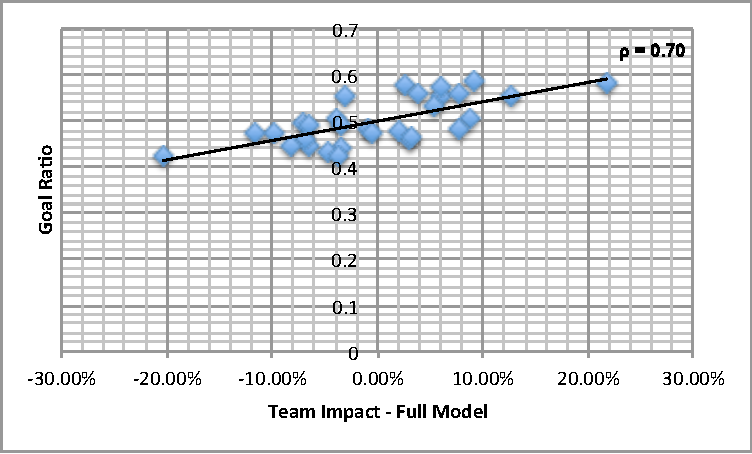
\includegraphics[width=0.7\textwidth]{impact-full}}
		\subfigure[Full look-ahead Without Location Information]{\label{fig:noloc-scatter}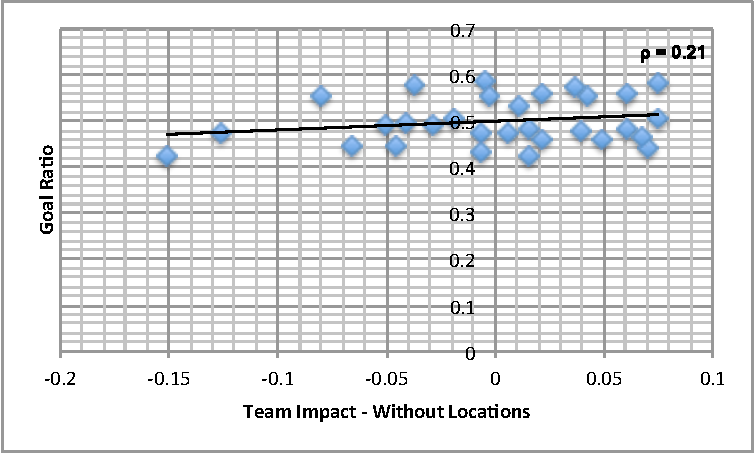
\includegraphics[width=0.7\textwidth]{impact-nolocation}}
		\subfigure[1-step look-ahead]{\label{fig:1step-scatter}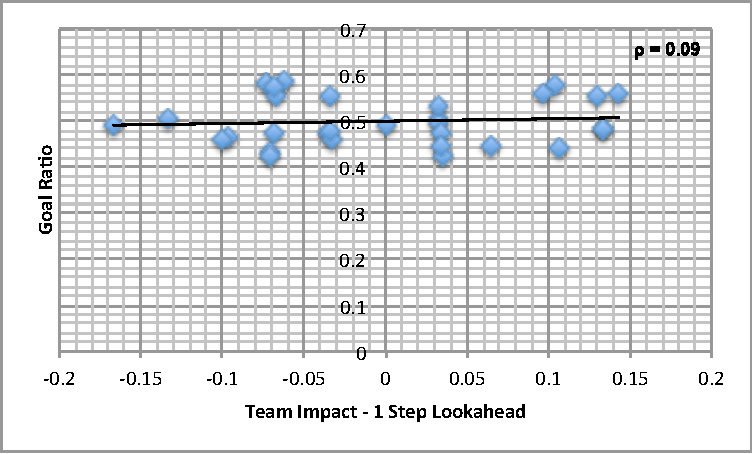
\includegraphics[width=0.7\textwidth]{impact-1step}}
		\subfigure[Average Value Difference]{\label{fig:value-diff}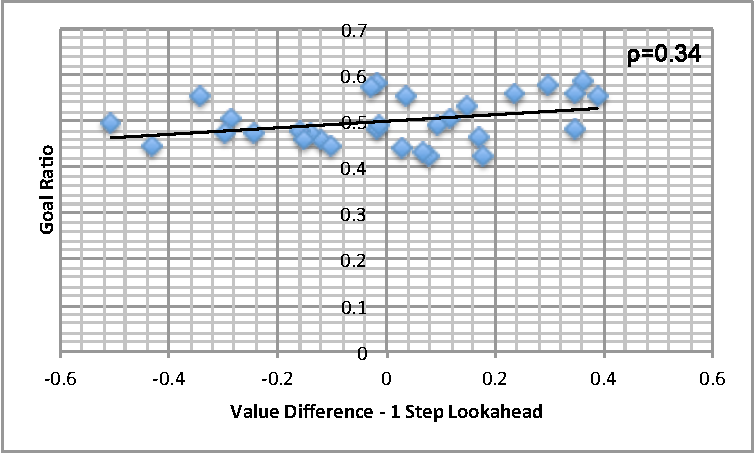
\includegraphics[width=0.7\textwidth]{value-diff}}
		\caption{Average Team Impact and Average Team Value Difference vs. Average Goal Ratio. Each datapoint represents a team. Action values are computed using the Next Goal reward function.}\label{fig:scatter}
	\end{figure}

\subsubsection{Correlations On Incomplete Datasets}

\paragraph{Single Game Outcomes} Figure~\ref{fig:single-match} shows the scatter plot for the correlation between goal ratio and the Team Impact in an individual match. The correlation coefficient is $\rho = 0.45$. This shows that impact values carry substantial information about the outcome of a match. An application may be to live betting during a match: The impact value total after, say, the first two periods may be good predictors of the final match outcome.

\begin{figure}
\centering 
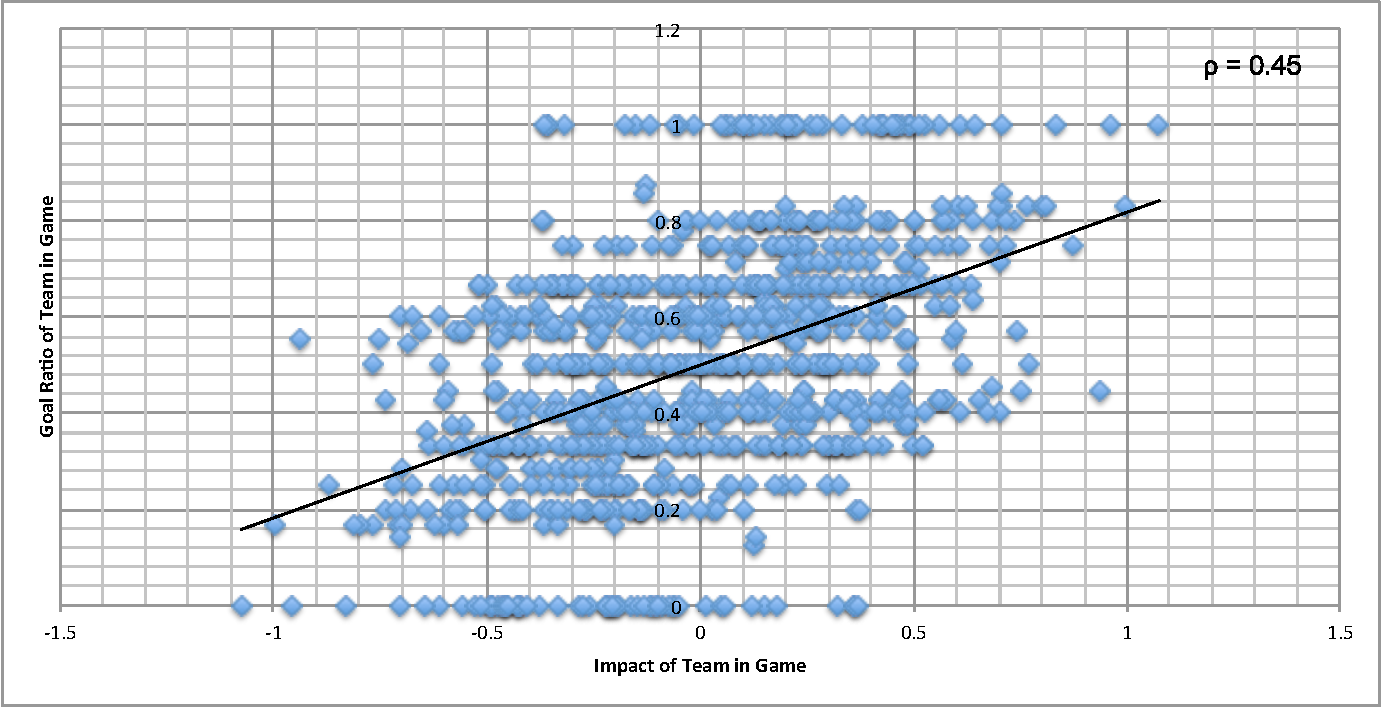
\includegraphics[width=1\textwidth]
{game-team-impact}
\caption{A team's Total Impact Values in a single match vs. the goal ratio result in that match. Each datapoint represents a pair (team-match).}
\label{fig:single-match}
\end{figure}


\paragraph{Final Goal Ratio From Initial Observations.} We also consider correlations computed not from the entire dataset, but from initial observations. Figure~\ref{fig:rounds} gives the correlation coefficients between the final Goal Ratio, averaged over all matches, and a moving average of the Team Impact Total, averaged over the first $k$ matches. The correlation is close to 0.5 after 10 matches, which is less than half the number of total matches for all teams in our dataset. This means that after a relatively small number of observed matches, the Average Team Impact carries substantive information about the final Goal Ratio performance of a team.

%We next apply the team performance estimated on the basis for team impact values to predict future performance in terms of goals. Following the methodology of \cite{Tegen2015}, we use a sliding window approach. Given a list of $k$ games, we find (1) the Total Value (Total Value Difference) for each team up to that point, and (2) the Number of Goals (Goal Difference) in the next game. A variant of this prediction used by \cite{Tegen2015} is to correlate estimated performance after $k$ games with the total goals from all games following. 

%\begin{figure}
%\centering     %%% not \center
%		\subfigure[Total Value/Total Value Difference vs. Goals/Goal Difference in Next Game]{\label{fig:nextgame}\includegraphics[width=0.48\textwidth]{missing}}
%		\subfigure[Total Value/Total Value Difference vs. Goals/Goal Difference in Following Games]{\label{fig:action1}\includegraphics[width=0.5\textwidth]{missing}}
%		\caption{The correlation between performance estimated using our model and future goal scoring performance. The $x = k$ shows the correlation after the first $k$ matches.}\label{fig:clustering}
%\end{figure}

\begin{figure*}
\centering 
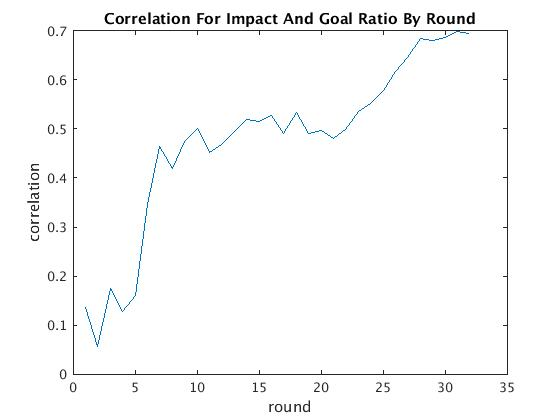
\includegraphics[width=1\textwidth]{correlation-by-round}
\caption{The correlation between Goal Ratio (averaged over all matches) and Team Impact (averaged over the first $k$ matches).}
\label{fig:rounds}
\end{figure*}

\subsection{Team Performance and State Values}

Another plausible approach to measuring team performance using a Markov model is to aggregate the team values for the states reached during the match. The intuition is that good teams manage maintain an advantage, that is, a higher chance of winning, for longer stretches than inferior teams. This motivates the \defterm{Average Team Value Sum} metric: For each game, sum the team values of the states reached during the match. Then average the summed values to obtain a team number for the whole dataset. With Next Goal as the reward function, the correlation with Goal Ratio is fairly weak, only 0.27. This is consistent with our previous result for the Average Team Value Difference (0.34): while achieving a relatively high likelihood of scoring is of course positively correlated with game outcome, it is a weak signal, compared with the ability to impact the scoring likelihood. However, this  changes when we use Win as the reward function rather than Next Goal. We refer to this special case of the Average Team Value Sum as the Average Team Winning Chance metric. For this metric, a high state value reflects the global likelihood of success in the overall game, not mainly in the current play only. Figure~\ref{fig:win-value-sum} shows that the ability to achieve many states with higher winning chance correlates strongly with goal ratio, with a correlation coefficient of 0.82.

\begin{figure}
\centering 
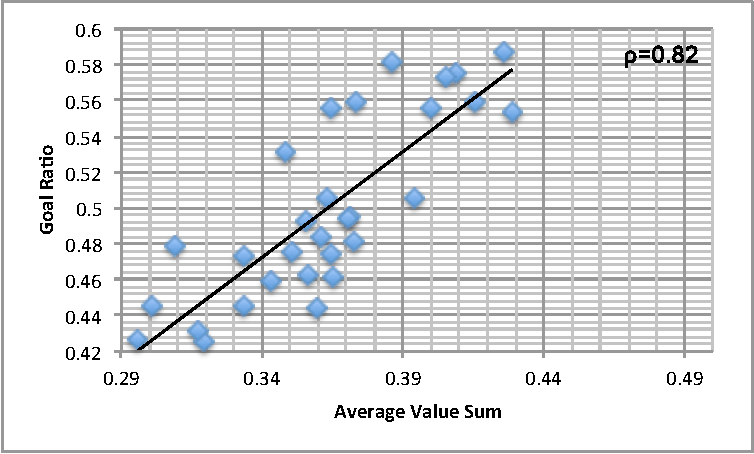
\includegraphics[width=1\textwidth]{value-sum-win}
\caption{The correlation between Goal Ratio (averaged over all matches) and the Average Winning Chance Metric, averaged over all matches. Each datapoint represents a team.}
\label{fig:win-value-sum}
\end{figure}



\section{CONCLUSION}

We have built  a large Markov Game Model for a large set of NHL play-by-play events with a rich state space. A novel aspect of our dataset is that it includes location information about where an action took place. 

Value iteration computes the values of each action ---the value function of the Markov game model. Compared to previous work that assigns a single value to actions, the Q-function incorporates two powerful sources of information for valuing hockey actions: (1) It takes into account the context of the action, represented by the Markov Game state. (2) It models the medium-term impact of an action by propagating its effect to future states. The value function provides knowledge about hockey dynamics by quantifying how much which action matters where.
%
We apply our model to evaluate the performance of teams in terms of their actions' total impact on which team scores the next goal.
%Action impact scores are calculated for players with respect to different objective functions.
The average impact score of a team for the next goal correlates highly with the team's average goal ratio ($\rho = 0.7$). An even higher correlation is achieved by the average team winning chance (0.82). 
In sum, the  value function is a powerful AI concept that captures much information about hockey dynamics as the game is played in the NHL.

\paragraph{Future Work} The NHL data provides a rich dataset for real-world event modelling. A number of further AI techniques can be applied to utilize even more of the available information than our Markov Game model does, especially for utilizing the spatio-temporal information. We mention two specific directions:

1) An {\em alternative discretization of locations} is to apply matrix factorization to a location transition matrix~\citep{Cervone2014a}. A cell in the transition matrix specifies the number of transitions from one location to another. (Given an initial fine-grained uniform discretization of locations to define rows and columns). Matrix factorization then produces a clustering of locations that models the information about which transitions are likely to occur: If two states are in the same cluster, their transition probabilities are the same. Our clustering based on location occurrence counts rather than transition counts is simpler and faster to compute, but does not utilize dynamic transition information.

2) We can utilize {\em process models with continuous time and space points}, rather than discretizing continuous quantities. 
%Space and time points can be included in a process model for continuous quantities rather than discretized. 
Continuous quantities include 
(i) the time between events, %---which requires a continuous time Markov Game model,
(ii) the absolute game time of the events, % (e.g. ``minute 15''),
(iii) unclustered location of actions. 
(The location of shots has been considered in previous work \citep{Krzywicki2005}.)  A promising model class are Piecewise Constant Conditional Intensity Models for continuous time event sequences \citep{Gunawardana2011,Parikh2012}. These models are especially well suited for sequences with a large set of possible events, such as our action events. 
% (however, reported shot locations are noisy ). % Player locations would be valuable information, but are currently not available for actions other than shots.

Our use of reinforcement learning techniques has been mainly for finding patterns in a rich data set, in the spirit of descriptive statistics and data mining. Another goal is to {\em predict} a player or team's future performance based on past performance using machine learning techniques. For example, can we predict a team's performance in the next match based on their performance in the previous ones? Or predict their final result in a match based on the first half of the match?
%Machine learning methods aim to provide reliable generalization, and can be combined with dynamic programming for predicting future performance \citep{bib:sutton}.
%For example, sequence modelling would be able to generalize from play sequence information. A
%A potential future application for improving play and advising coaches is in finding strengths and weaknesses of teams: We can use the value function to find situations in which a team's mix of actions provides a substantially different expected result from that of a generic team.



\subsubsection*{Acknowledgements} This work was supported by an Engage Grant from the National Sciences and Engineering Council of Canada. We are grateful for constructive discussions in SFU's Sports Analytics Research Group. 
\newpage

%\subsubsection*{Acknowledgements}

%Use unnumbered third level headings for the acknowledgements title.
%All acknowledgements go at the end of the paper.


%\subsubsection*{References}

%References follow the acknowledgements.  Use unnumbered third level
%heading for the references title.  Any choice of citation style is
%acceptable as long as you are consistent.

%NOTE: NEED TO USE CORRECT REFERENCES HEADER
\bibliographystyle{apalike}
\renewcommand\bibsection{\subsubsection*{\refname}}
\bibliography{master-dmkd}


%J.~Alspector, B.~Gupta, and R.~B.~Allen  (1989). Performance of a
%stochastic learning microchip.  In D. S. Touretzky (ed.), {\it Advances
%in Neural Information Processing Systems 1}, 748-760.  San Mateo, Calif.:
%Morgan Kaufmann.

%F.~Rosenblatt (1962). {\it Principles of Neurodynamics.} Washington,
%D.C.: Spartan Books.

%G.~Tesauro (1989). Neurogammon wins computer Olympiad.  {\it Neural
%Computation} {\bf 1}(3):321-323.

\end{document}
